\documentclass[fontset=macnew,UTF8]{article} % 12pt 为字号大小 UTF8
\usepackage{ctex}
\usepackage{amssymb,amsfonts,amsmath,amsthm}
\newtheorem{theorem}{Theorem}
\newtheorem{definition}{Definition}
\usepackage[linesnumbered,ruled,vlined]{algorithm2e}
\usepackage{arevmath}  % 数学符号
\usepackage{color}
%\usepackage{fontspec,xltxtra,xunicode}
%\usepackage{times}

%----------
% 定义中文环境
%----------

\usepackage{xeCJK}

% \setCJKmainfont[BoldFont={SimHei},ItalicFont={KaiTi}]{SimSun}
% \setCJKsansfont{SimHei}
% \setCJKfamilyfont{zhsong}{SimSun}
% \setCJKfamilyfont{zhhei}{SimHei}

% \newcommand*{\songti}{\CJKfamily{zhsong}} % 宋体
% \newcommand*{\heiti}{\CJKfamily{zhhei}}   % 黑体


%----------
% 版面设置
%----------
%首段缩进
\usepackage{indentfirst}
\setlength{\parindent}{2.1em}

%行距
\renewcommand{\baselinestretch}{1.4} % 1.4倍行距

%页边距
\usepackage[a4paper]{geometry}
\geometry{verbose,
  tmargin=3cm,% 上边距
  bmargin=3cm,% 下边距
  lmargin=3cm,% 左边距
  rmargin=3cm % 右边距
}


%----------
% 其他宏包
%----------
%图形相关
\usepackage[x11names]{xcolor} % must before tikz, x11names defines RoyalBlue3
\usepackage{graphicx}
\usepackage{pstricks,pst-plot,pst-eps}
\usepackage{amsmath,amssymb,amsfonts, amsthm}
\usepackage{float}
%\usepackage{subfig}
\def\pgfsysdriver{pgfsys-dvipdfmx.def} % put before tikz
\usepackage{tikz}
\usepackage{cite}
\usepackage{threeparttable}
\usepackage{diagbox}
%原文照排
\usepackage{verbatim}
\definecolor{gray}{gray}{0.9}
\usepackage{multirow}
%网址
\usepackage{url}
\usepackage{framed}
\usepackage{subfigure}
\usepackage{xcolor}
\usepackage{colortbl}
\usepackage{booktabs} 
\usepackage{caption}

\newcommand{\redstar}{{\color{red}{$\bigstar$}}}
\newcommand{\cyanlozenge}{{\color{cyan}{$\blacklozenge$}}}
\newcommand{\yellowtriangle}{{\color{black!30!green}{$\blacktriangle$}}}

\newcommand{\horrule}[1]{\rule[0.5ex]{\linewidth}{#1}} 	% Horizontal rule

\renewcommand{\refname}{参考文献}
\renewcommand{\abstractname}{\large \bf 摘\quad 要}
\renewcommand{\contentsname}{目录}
\renewcommand{\tablename}{表}
\renewcommand{\figurename}{图}


\setlength{\parskip}{0.4ex} % 段落间距

\usepackage{enumitem}
\setenumerate[1]{itemsep=0pt,partopsep=0pt,parsep=\parskip,topsep=5pt}
\setitemize[1]{itemsep=0.4ex,partopsep=0.4ex,parsep=\parskip,topsep=0.4ex}
\setdescription{itemsep=0pt,partopsep=0pt,parsep=\parskip,topsep=5pt}


\begin{document}

\title{
{\textsc{
南京大学\\
计算机系技术报告 \\[150pt]}}
\horrule{2.5pt}\\
\sffamily{复杂环境下的深度学习模型融合与测试技术研究}
\horrule{1.8pt}\\[150pt]
}
%\author{姓名\quad 孟令涵\\menglinghan@smail.nju.edu.cn}
\date{2024年3月} % 若不需要自动插入日期,则去掉前面的注释;{ } 中也可以自定义日期格式

\begin{titlepage}
\maketitle
\vspace{30pt}
\thispagestyle{empty}
\end{titlepage}

\tableofcontents
\thispagestyle{empty}

\newpage
\setcounter{page}{1}

\section{研究背景及意义}
% 研究的应用背景(实际的问题,引出研究的东西)
近年来,深度学习模型在许多安全攸关场景中广泛应用,如医疗\cite{medical}、自动驾驶\cite{self_Driving}和语音识别\cite{speech_recognition}等领域。在这些复杂应用环境下,虽然深度学习模型已达到甚至超越人类的能力,但深度学习模型在开发维护\cite{menghani2023efficient}和质量保障\cite{chakraborty2019software}等方面中仍然面临挑战。在深度学习模型开发方面,正如在文献\cite{mohammed2023comprehensive}中所述,深度学习模型的训练过程需要付出巨大的努力,调整最优超参数需要专业知识和大量的尝试,这是一项繁琐且耗时的任务。在质量保障方面,例如,Tesla的自动驾驶汽车事故就造成了人员财物上的巨大损失\cite{Tesla}。因此,迫切需要相应的技术去提高深度学习模型开发维护效率和安全性以应对复杂的应用和开发环境。

% 解释研究的东西是什么(深度学习模型的开发与维护和质量保障)
深度学习模型开发与维护:开发和维护深度学习模型的主要挑战之一是模型训练,这通常需要大量的人力资源和计算能力(如标记成本和参数训练)。深度学习模型质量保障:涵盖模型质量的多方面指标,包括正确性和安全性等\cite{landscapes}。和传统软件相比,深度学习模型的正确性和安全性范畴具有很大的不同。传统软件程序主要依赖于程序员手动构建业务逻辑,深度学习模型主要通过数据驱动的编程范式来构建,其决策逻辑通过训练过程来获得,即模型的行为可能会随着新的训练数据的加入而演化\cite{amershi2019software}。除源代码之外,训练数据集和模型是影响深度学习系统质量的重要组成部分。

% 研究的技术(DL testing)现状
软件复用是提高软件开发维护的常用方法,通过复用已经已有的代码,进而提高开发维护效率\cite{poulin1996measuring}。深度学习模型复用技术,尝试复用现有的可用的在其他任务上训练的模型来构建模型,这为减少所需的训练样例数量和训练时间成本提供了巨大的潜力,因为现有模型的利用可能有助于为新模型的训练奠定良好的基础。近年来,在深度学习模型复用领域,学者们进行了广泛研究。文献\cite{zhou2016learnware}强调可重用性是学习软件新概念的一个关键特征。如果模型可以在与原始训练场景有很大不同的场景中重用,那该模型具有良好的可重用性。随着深度学习的快速发展,开发者发布了越来越多的预训练模型。经过训练的模型可以被视为相应任务的专\cite{yang2017deep}. 如何复用模型中包含的知识引起了学者们的关注。模型融合技术提供了模型知识复用的可能技术。You等\cite{you2017learning}提出了一种从多个教师模型中提取知识来训练学生模型的方法。在进行知识融合时,不仅要考虑实际教师模型的输出,还要考虑模型中间层不同样本的表示。Shen等\cite{shen2019amalgamating}提出通过知识合并完成综合分类任务,但限制教师模型必须是同构的。在进一步的研究中,Shen 等\cite{shen2019customizing}提出通过知识合并从异构教师模型中获得学生模型。

软件测试是软件质量保障的常用方法,通过暴露和修复软件系统问题,进而提高软件系统的质量\cite{landscapes}。深度学习模型的统计特性为深度学习模型测试和增强带来了新的问题和挑战。近年来,在深度学习测试领域,学者们进行了广泛的研究。深度学习模型的测试问题,可以被描述为测试的工作流程(如何去测试)、测试属性(为什么去测试)以及测试组件(去哪里测试和测什么)。对于安全性的测试旨在尽可能高效的找出模型的错误,Pei等\cite{pei2017deepxplore}提出的一种白盒测试技术DeepXplore,通过筛选较高神经元覆盖率的输入样本,触发了自动驾驶学习系统中数以千计的错误驾驶行为。Tian等\cite{tian2018deeptest}提出了DeepTest,该方法使用九种不同的真实图像变换执行贪婪搜索,在Udacity自动驾驶数据挑战集上检查出1,000多个深度学习模型的错误。深度学习模型增强的研究主要集中在训练数据集精化和深度学习模型的权重数值方面\cite{shen2020mcp}。数据质量对模型的质量有着重要的影响:即使拥有再好的深度学习模型结构,没有好的训练数据也无法很好地执行。尽管深度学习通常被认为是一种依赖“大”数据的方法,但深度学习模型的测试通常受到有限标记代价的限制,因此它必须采用具有统计效率的“小”数据方法\cite{Boosting}。如何在有限标记代价下更好地增强模型的性能,引起学者们的广泛关注。Feng等\cite{feng2020deepgini}一种黑盒测试技术DeepGini, 该方法选择重训练样本对模型进行重训练来增强模型。

%综上,提出我们要去解决的问题
综上所述,深度学习的模型融合与测试技术是保障开发效率和安全性的两个重要环节,当将深度学习模型视为一种新型软件时,研究强调软件工程 可以帮助开发深度学习模型并提高其质量,即是时候强调软件工程对于 深度学习\cite{menzies2019five}的重要性了。通过模型融合技术提高模型开发和维护效率,通过深度学习测试技术发现模型的缺陷。本文针对深度学习模型融合和测试开展了两项工作:

第一个研究问题:我们从一个新的应用场景来研究深度学习模型融合技术,开发和维护深度学习模型的主要挑战之一是训练深度学习模型非常昂贵,特别是对于具有数十亿参数和大型数据集的模型\cite{li2021modeldiff,shen2020mcp}。 解决这个问题的软件工程方法是借鉴传统软件重用实践的思想\cite{poulin1996measuring},即复用深度模型\cite{pan2022decomposing,meng2021measuring}。当前的模型重用研究包括两个方面:模型切片\cite{zhang2022remos}和模型模块化\cite{pan2020decomposing,qi2022patching},两者都旨在减少深度学习模型以适应给定任务的特定要求。 隐藏的逻辑是,如果深度学习模型配备了过多的功能(即,可能只需要模型功能的一小部分来解决目标问题的要求),就会导致更长的推理时间和运行成本。 因此,首选重用与特定问题相关的训练模型的某些组件\cite{qi2023reusing}。

与之前的软件工程研究不同,我们关注的是更复杂的重用场景,需要重用多个深度学习模型。正如\cite{meng2021measuring}中所述,随着模型构建和共享技术的成熟,产生了多个具有相似功能的深度学习模型 ,即功能重叠。面对如此多种DL模型,开发人员可能需要将它们组合起来,构建联合模型来实现统一的需求。 具体来说,以我们研究的真实数据集为例,图 1 显示有两个深度学习模型 A 和 B,其目标是将输入分类为各种动物。 如图 1 所示,模型 A 和 B 具有功能重叠,即两者都可以识别猫和狗的输入。 此外,我们注意到模型A(B)有其独特的输出类别,熊猫(大象、马和狮子)。 这个例子说明了一个更复杂的重用场景:当所有输出类别都被视为新深度学习模型的功能需求时,开发人员将致力于组合现有深度学习模型(即连接模型 A 和 B)来构建联合模型(即模型 C 如图 1 所示)以及所有输出类别。

\begin{figure}[h]
	\centering
	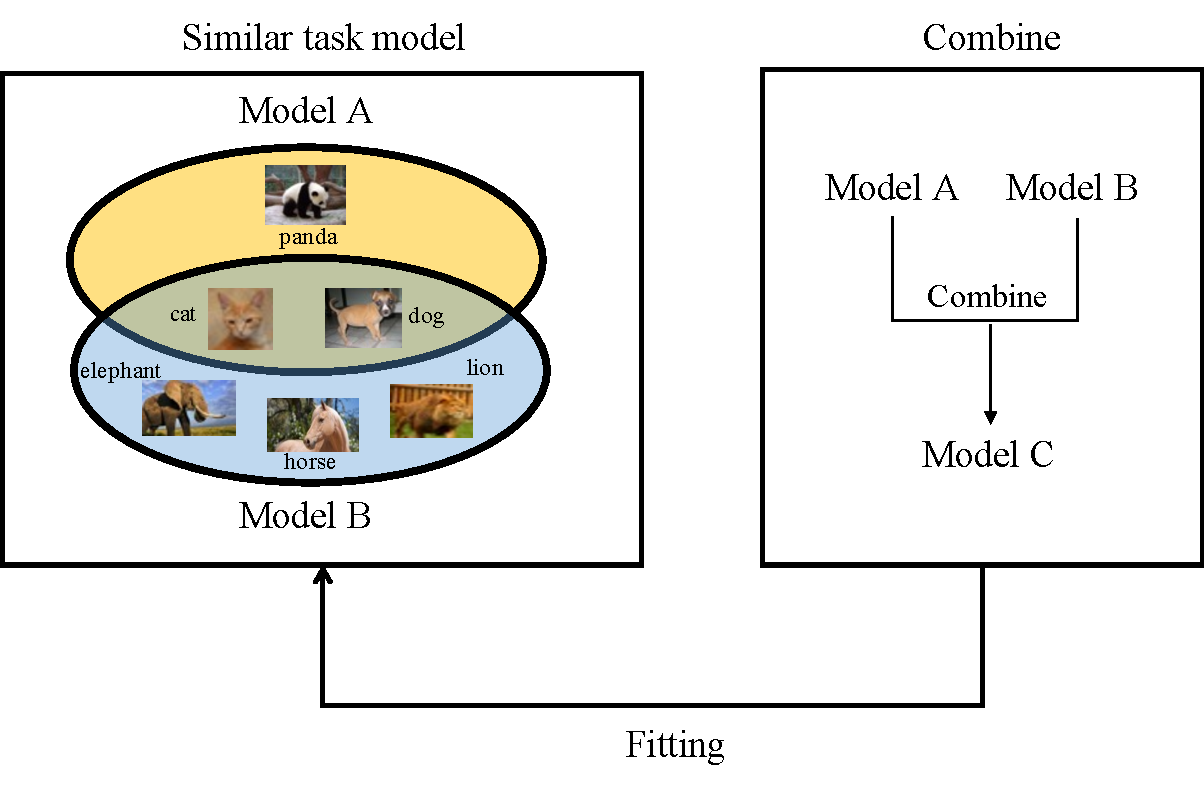
\includegraphics[width=0.5\linewidth]{MCCP_scene.pdf}
	\caption{这是一个展示我们研究场景的示例,开发人员旨在组合两个深度学习模型(模型 A 和 B)来构建联合模型(模型 C)。}
	\label{MCCP}
\end{figure}

从软件工程的角度来看,我们指出了结合深度学习模型来满足新需求时的两个局限性。
\begin{itemize}
	\item 在实际应用中,我们通常只能获得多个模型(即模型文件)作为研究对象,而没有它们的训练数据集,这阻碍了从训练数据集构建新的联合模型
	 \item  组合深度学习模型需要来自应用程序上下文的标记数据。 由于人工标记的成本很高,标记的数据是有限的,即应用上下文中的一小部分样本可以被标记。
\end{itemize}

为了解决上述限制,我们的研究密切关注“如何以有限的标记工作从应用程序上下文中提取信息”,分为两个步骤。 首先,我们从 Kaggle 平台收集数据和模型,并进行实证研究,观察具有重叠功能的多个 DL 模型的性能,这提出了组合多个模型的需求。 其次,我们提出了基于级联并行的模型组合方法,称为MCCP。 为了探讨模型组合在这种场景下的好处以及MCCP是否可以有更好的性能,我们组织实验来回答以下两个研究点:

\begin{itemize}
	\item \textbf{研究点1(Why):重叠类别数据中多个模型的性能是否存在明显差异?} 
	
	实验结果显示两个重叠类别的数据分布存在差异(约1\%到38\%)。通过模型组合可以满足全分类要求。
	
	\item  \textbf{研究点2(How):我们的方法比基线更有效吗?} 
	
	在收集到的数据集上,我们训练了不同采样率下的学生模型,评估了混合测试集上的分类精度,将 MCCP 与三个基线进行了比较,发现在大多数情况下(9 个 场景中的 8 个场景)MCCP 优于基线。
\end{itemize}

本研究问题的主要贡献如下:

\begin{itemize}
	\item 我们提出了一种简单直接的模型融合方法,称为MCCP,它通过组合训练好的模型来生成组合模型,并以有限的标记成本更好地训练联合模型以覆盖整体分类
	\item  	我们对模型组合技术进行了实证研究,将MCCP 与九个不同领域分类数据集上的三个基线进行了比较。 实验结果表明,MCCP非常有效,即可以在有限的标记成本下对总体混合数据进行分类,并且与基线相比具有更好的性能。
\end{itemize}





第二个研究问题,对于深度学习模型测试,我们主要关注深度学习模型后门防御研究。由于深度神经网络模型通常采用一些来自不可信第三方的外部训练数据,因此强大的后门防御策略非常重要。我们认为防御的核心是从中毒的训练集中将中毒样本识别出来。

一些恶意的攻击者对深度学习模型植入后门\cite{liu2020survey,kaviani2021defense,li2022backdoor},使得模型的预测结果与实际结果产生差异。由于深度学习模型通常被看做黑盒子,其内部逻辑很难被理解,因此深度学习模型的后门很难被发现与修复,对模型的准确性和安全性产生了很大的影响。学者们为了缓解后门攻击带来的影响提出了一系列防御方法。现有的方法大多只针对单一目标类后门的攻击进行防御。大体可以分为模型防御和输入防御两大类。在模型防御方面:Liu等\cite{liu2019abs}提出名为ABS的技术,用于扫描深度学习模型以检测是否被植入了后门;在输入防御方面:Gao等\cite{gao2019strip}提出名为STRIP技术,它是一个基于强烈的故意扰动的运行时木马攻击检测系统。具体来说,其通过故意扰乱被检测的输入,例如叠加各种图像模式,并观察预测的扰动输入的类别,预测类别中的低熵意味着存在木马输入的特征。基于以上的研究,我们针对输入防御方面提出基于熵的木马输入检测ETID(Entropy-based Trojaned Input Detection)我们的方法与先前的检测技术在视角上有明显的区别:1)我们的假设是木马样本对模型决策边界更不敏感;2)我们采用变异测试技术对$\mathcal{M}_\mathcal{I}$进行变异,以修改其决策边界。我们在三种广泛应用的数据集和六种攻击操作的场景下对ETID进行了评估,实验结果表明我们提出的检测方法对木马输入样本检测是有效的。

本文后续内容按如下结构进行组织:第二章介绍深度学模型测试和增强技术的相关工作;第三章对解决的两个问题进行描述;第四章提供了对于两个问题的解决思路和方案;最后一章对已完成的研究工作进行总结并规划未来的研究计划。

\section{相关工作}
本章介绍与深度学习模型融合和测试技术相关的工作,主要从深度学习模型模型融合技术和深度学习模型测试技术两个部分进行介绍。

\subsection{深度学习模型融合}
\subsubsection{知识复用}
随着深度学习的快速发展,开发者发布了越来越多的预训练模型。 一个经过训练的模型可以被视为其相应任务的专家\cite{yang2017deep}。如何重用模型中包含的知识引起了学者们的关注。 对此,我们从以下三个方面介绍相关工作:模型重用、知识蒸馏和知识融合
\subsubsection{模型重用}
 从模型池中选择对当前任务有帮助的模型进行复用,是模型复用的关键一步。 Ding等人\cite{ding2020boosting} 研究了从模型池中选择模型子集来对未标记的数据集进行分类,而无需访问模型的原始训练数据。 Meng等人\cite{meng2021measuring}提出了一种可以以有限的标记成本对源模型进行排序的方法,以从具有相同功能的多个模型中选择更适合目标任务的模型。Zhang等人\cite{zhang2021towards}研究了模型池中的模型如何在不完全覆盖目标任务的情况下识别出对目标任务有价值的模型。 Wu等人\cite{wu2021model}人研究了如何在不访问模型池中模型的原始训练数据的情况下从模型池中选择满足当前任务的模型,他们提出了一个两阶段框架。 基于此,Tan等人\cite{tan2022towards} 进行了进一步的研究,特别是考虑到各种预训练模型通常是从现实场景中的不同特征空间获得的。 这是使多路复用模型能够处理异构特征空间的首次尝试。 Ding等人\cite{ding2022pre}研究了迁移学习领域开源预训练模型的可重用性评估,提出了适用于一般学习任务的协同学习算法和模型。

相应地,近年来也提出了一些模型重用方法。 Wu等人\cite{wu2019heterogeneous}提出了一种称为HMR的通用异构模型重用,用于有限通信成本(即有限的标记训练样本)下的多方学习。 Zhao等人\cite{zhao2020handling}提出了一种通过模型重用来处理概念漂移的方法。 Shao等人\cite{shao2021towards}提出了使用多潜在域方法的模型重用,以解决来自目标任务中潜在未知域的数据问题。 Pan等人\cite{pan2022decomposing}提出了模型分解的方法,提高了模型开发的可重用性、可替换性和模块化程度。 Qi等人\cite{qi2022patching}。通过卷积神经网络的模块化和组合来增强神经网络。

同时,模型复用也会带来一些问题。 Ji等人\cite{ji2018model}。研究了模型重用带来的安全问题,并提出了一种广泛的模型重用攻击方法。 分析表明,复用模型前所未有的复杂性是安全问题产生的原因,并给出了潜在的对策和相应的挑战。模型复用还可能导致漏洞传播,因此Li等人提出了模型复用可能导致漏洞传播的问题。 \cite{li2021modeldiff}提出了ModelDiff,一种基于测试的深度学习模型相似度比较方法,用于模型重用检测。 减轻迁移学习中模型重用导致的漏洞或后门的继承。 Zhang等人\cite{zhang2022remos}。提出了模型切片技术来继承更多相关权重以减少缺陷继承。 Qi\cite{qi2023reusing}等人。提出了模型重组的概念,设计了提高模型复用性的工具,以缓解模型复用带来的缺陷继承。
\subsubsection{知识融合}
知识融合的主要目的是整合教师模型中包含的暗知识,获得多功能的学生模型。 You等人\cite{you2017learning}提出了一种从多个教师模型中提取知识来训练学生模型的方法。 在进行知识融合时,不仅考虑实际教师模型的输出,还考虑模型中间层不同样本的表示。 Shen等人\cite{shen2019amalgamating}提出通过知识融合来完成综合分类任务,但限制了教师模型的同质性。 在进一步的研究中,Shen 等人\cite{shen2019customizing}提出通过异构教师模型的知识融合来获得学生模型。 Ye等人\cite{ye2019amalgamating}通过融合来自教师模型的过滤知识,使学生模型掌握教师模型的全部或子集经验。 Ye等人\cite{ye2019student} 个融合了两个不同侧重点的教师模型的知识,用于训练多功能学生模型。 Liu等人\cite{liu2019knowledge}提出了从教师模型到学生模型的知识流,性能超过微调。 Jing等人\cite{jing2021amalgamating} 提出了一种图神经网络中知识融合的方法。 Yu等人\cite{yu2022arm} 通过知识融合使神经检索模型对新旧数据更加准确。Xu等人\cite{xu2022hierarchical}提出了双重判别特征对齐(DDFA)框架来改善类外类别的知识融合。Carvalho等人\cite{de2022class}通过知识融合缓解了神经网络的灾难性遗忘问题。
\subsubsection{知识蒸馏}
知识蒸馏与知识融合类似,但它侧重于通过蒸馏过程将教师模型的知识转移到学生模型。 近年来模型蒸馏的工作大致可以分为以下几个方面。多师模型蒸馏\cite{zhao2020highlight,park2020feature}。 缓解教师模型和学生模型在结构和数据层面的匹配问题\cite{zhu2021student,mirzadeh2020improved,fang2021mosaicking}. 回顾文献\cite{wang2021knowledge,gou2021knowledge}并提出一些新的知识蒸馏方法\cite{li2022distilling,chen2022knowledge}.

\subsection{深度学习模型测试}
目前深度学习模型测试旨在通过实施不同的深度学习测试技术来检测模型的质量。Pei等\cite{pei2017deepxplore}提出了一种名为DeepXlpore的白盒测试技术,是基于神经元覆盖的测试。揭示了自动驾驶学习系统中数以千计的错误转弯行为。Moosavi-Dezfooli等\cite{moosavi2016deepfool}提出名为DeepFool的测试鲁棒性技术,通过添加愚弄深度学习模型的噪音去评估该模型的鲁棒性。Carlini and Wagner等\cite{carlini2017towards}使用距离度量量化相似性的来生成对抗样本。Papernot等\cite{goodfellow2016cleverhans,papernot2016technical}设计了一个库来标准化来生成对抗样本。Zhang等\cite{zhang2018empirical}通过实证研究发现发现175个模型错误中有9个(5.1\%)属于效率问题。这个比例不高。原因可能是效率问题很少发生,或者这些问题很难检测。AEQUITAS\cite{saleiro2018aequitas}是一种公平性测试技术,它的目标是在数据集中发现存在偏见的实例,并据此生成更多的测试用例来帮助模型进行再训练。Doshi-Velez等\cite{doshi2017towards}给出了可解释性评估(测试)方法的分类:基于应用程序、基于人和基于功能。Ding等\cite{ding2018detecting}将程序视为灰色框,并通过统计测试来检测不同的隐私侵犯行为。Ahuja等\cite{ahuja2022testing}对多种深度学习模型测试技术进行了比较。

传统的变异测试技术也被拓展用于深度学习测试。Shen等人最先提出了MuNN技术\cite{shen2018munn},首次将变异测试技术应用于不同类型的深度学习模型,并提出了五种变异算子。Ma等在DeepMutation 方法\cite{ma2018deepmutation}中提出了更丰富的变异算子,包括模型级和源码级,并通过实验证明了变异测试技术在深度学习软件中的有效性。Hu等人\cite{hu2019deepmutation++}推出了一个升级的变异测试工具DeepMutation++,它不仅支持正常的深度神经网络,还支持有状态的循环神经网络(RNN)。Hildebrandt 等认为目前的变异算子无法模拟实际故障的影响,他们通过对深度学习软件实际故障的实证研究,在工具DeepCrim额\cite{humbatova2021deepcrime}中实现了24 个深度学习变异算子,这是基于真实错误的源代码级预训练变异工具。他们的实验也显示DeepCrime 对测试数据质量变化的敏感性优于DeepMutation++。
	


\section{问题描述}
本文对深度学习模型融合与测试技术展开研究,关注深度学习模型合并和后门样本检测两个问题,并对两个问题给予了解决方案。下文将对本文研究的问题进行描述。

\subsection{模型融合}
由第一章所述,我们的研究方向是,在图像分类任务中我们将两个分类功能具有重叠的模型进行合并,来增强神经网络模型,使合并模型可以满足全分类任务需求。在此我们对此研究问题进行具体描述。

如下图\ref{moti2}所示,给定两个分类任务,分别记为Task $\mathcal{T}_\mathcal{A}$ 和Task $\mathcal{T}_\mathcal{B}$,其中$\mathcal{T}_\mathcal{A}$ 的类别空间为$\mathcal{C}_1, \mathcal{C}_2, \mathcal{C}_3, \mathcal{C}_4$ 记为 $\mathcal{C_A}$ ,$\mathcal{T_B}$ 的类别空间为$\mathcal{C}_3, \mathcal{C}_4, \mathcal{C}_5, \mathcal{C}_6$ 记为 $\mathcal{C_B}$ ,并且它们是重叠的,即$\mathcal{C_A}\cap \mathcal{C_B} =   {{\mathcal{C}_3,\mathcal{C}_4}}$。$\mathcal{M_A}$ 是在$\mathcal{T_A}$上训练的模型 ,$\mathcal{M_B}$是在Task $\mathcal{T_B}$.上训练的模型。 
通过对$\mathcal{M_A}$和$\mathcal{M_B}$进行融合生成$\mathcal{M_C}$可以满足新的分类任务Task $\mathcal{T_C}$ ,其应用上下文有大量未标记数据,其类别空间$\mathcal{C_C = C_A \cup C_B}$。

\begin{figure}[h]
	\centering
	\begin{tabular}{|c|c|c|c|c|c|c|c|}
		\hline
		\multirow{2}*{模型} & \multicolumn{6}{c|}{类别空间} & \multirow{2}*{任务}\\
		\cline{2-7} 
		& $c_1$ & $c_2$ & $c_3$ & $c_4$ & $c_5$ & $c_6$  & \\
		\hline 
		\hline
		$\mathcal{M_A}$ & \checkmark  & \checkmark  & \checkmark  & \checkmark  & $\times$ & $\times$ & $\mathcal{T_A}$ \\
		\hline 
		$\mathcal{M_B}$ & $\times$ & $\times$  & \checkmark &  \checkmark& \checkmark & \checkmark  & $\mathcal{T_B}$ \\
		\hline 
		$\mathcal{M_C}$ & \checkmark  & \checkmark &  \checkmark & \checkmark & \checkmark  & \checkmark & $\mathcal{T_C}$ \\
		\hline 
	\end{tabular}
	\caption{模型合并的例子。 \checkmark 和 $\times$ 代表了是否包含分类。}
	\label{moti2}
\end{figure}

由于数据隐私的保护或其他一些场景限制,我们假设无法获取$\mathcal{T_A}$和 $\mathcal{T_B}$ 的训练数据集。 只能得到训练好的模型$\mathcal{M_A}$和$\mathcal{M_B}$。 由于人工注释的成本,只能标记少量数据。 因此,如何在有限的标记数据下重用$\mathcal{M_A}$和$\mathcal{M_B}$更好地解决$\mathcal{T_C}$的分类任务是我们研究的主要问题。

很多应用场景都满足上述假设。 以医院对一组特定疾病的分类为例。 $\mathcal{C}$医院,拥有大量未标记的疾病图像。 迫切需要对这些图像进行分类,类别空间被认为是$\mathcal{C_C}$。另外还有两家医院:(a)医院$\mathcal{A}$建立了$\mathcal{M_A}$,可以用类别空间$\mathcal{C_A}$对分类法的部分进行分类,(b)医院$\mathcal{B}$有$\mathcal{M_B}$,可以对疾病的分类法和类别空间的部分进行分类$\mathcal{C_B}$。出于保护患者隐私的考虑,$\mathcal{C}$医院只能获取$\mathcal{A}$医院和$\mathcal{B}$医院的模型,而无法获取相应的训练数据。而且,由于标注疾病图片需要专业医生,标注成本较高。因此,在标记样本有限的情况下,如何复用$\mathcal{M_A}$和$\mathcal{M_B}$来满足医院$\mathcal{C}$任务是一个非常现实的需求。

\subsection{后门模型木马输入检测}
由第一章所述,深度学习测试技术普遍用于揭露模型的问题。可以利用测试技术来对被植入后门的模型进行木马样本检测。在此我们给出三个定义来说明要解决的问题。

\begin{definition}[深度学习模型]
深度神经网络结构实现的深度学习模型可以被看做一个复杂分类器。该分类器实现了特征域 $F_d$ 到分类域$C_d$的映射,$\mathcal{M}: F_d\rightarrow C_d$,当一个入$x\in F_d$ 是特征向量,那么对应的输出$y\in C_d$, 其中$C_d=\{C_1,C_2,...,C_m\}$。
\end{definition}

\begin{definition}[后门攻击和目标类]
后门攻击通过将隐藏的后门植入到原始深度学习模型$\mathcal{M}_\mathcal{O}$ 的模型结构中来感染模型。判断后门攻击成功与否,要看是否满足下面两点:\textbf{(a)}
在干净(正常样本)$x^c$输入下,被植入的深度学习模型 $\mathcal{M}_\mathcal{I}$ 行为不改变 , 即, $\mathcal{M}_\mathcal{I}(x^c)=\mathcal{M}_\mathcal{O}(x^c)$; 
\textbf{(b)} 
当后门被攻击触发器激活后,$\mathcal{M}_\mathcal{I}$ 预测木马输入 $x^t$ 为攻击指定的分类\textbf{目标类别} $C_\mathcal{T}$, 即,  $\mathcal{M}_\mathcal{I}(x^t)=C_\mathcal{T}$。
\end{definition}

\begin{definition}[木马输入检测]
给定一个被感染深度学习模型$\mathcal{M}_\mathcal{I}$ 和一个包含干净和恶意样本输入的集合$\{x_1,x_2,\dots,x_n\}$,假定当前模型不知道被植入后门的攻击和目标类信息。我们要研究的问题如下:对于每一个输入样本${x_i}$,可以检测出$x_i$是否是木马输入。即,$\text{TID}(x_i)\in \{\text{clean},\text{trojaned}\}$。
\end{definition}

我们将采用软件测试的思路去研究木马输入检测的问题,具体为采用深度学习变异测试技术来生成被感染模型的变异体,通关观察变异体在木马输入和干净输入的差异来识别木马输入。


\section{思路及解决方案}
本章中将对第三章提出的两个问题提供思路及解决方案。

\subsection{基于级联并行的模型合并技术}
\textbf{数据集:}我们从 Kaggle 平台收集了 9 对 18 个数据集进行实证实验。 我们收集的数据集具有三个特征。首先,我们关注图像分类数据集。其次,分类任务的领域广泛,涵盖不同的应用领域,例如汽车、花卉、水果等。每对数据集对应一个领域,其中包含$\mathcal{T_A}$和$\mathcal{T_B}$。第三,品类重叠。例如,在汽车领域,$\mathcal{T_A}$有7个类别,$\mathcal{T_B}$有8个类别,并且有五个类别重叠。

% Please add the following required packages to your document preamble:
% \usepackage{multirow}

	\begin{table}[t]
		\renewcommand\arraystretch{1.2}
		\centering
		\caption{The datasets and models used in this experiment.}
		\label{dataset}
		\scalebox{0.6}{
			\begin{tabular}{|l|l|l|c|c|cc|cc|}
				\hline
				\multirow{2}{*}{领域}    & \multirow{2}{*}{数据集}                   & \multirow{2}{*}{模型} & \multirow{2}{*}{类别数} & \multirow{2}{*}{重叠数} & \multicolumn{2}{c|}{性能}          & \multicolumn{2}{c|}{数据量}                                        \\ \cline{6-9} 
				&                                            &                        &                             &                                         & \multicolumn{1}{c|}{训练集准确率} & 测试集准确率 & \multicolumn{1}{l|}{训练集数据量} & \multicolumn{1}{l|}{测试集数据量} \\ \hline \hline
				\multirow{2}{*}{Car}       & Car Body Style Dataset~\cite{CarBodyStyleDataset}                     & Xception               & 7                           & \multirow{2}{*}{5}                      & \multicolumn{1}{c|}{0.964}     & 0.8125   & \multicolumn{1}{c|}{2670}       & 672                            \\ \cline{2-4} \cline{6-9} 
				& Car Body Style~\cite{CarBodyStyle}                             & Xception               & 8                           &                                         & \multicolumn{1}{c|}{0.9675}    & 0.815    & \multicolumn{1}{c|}{1599}       & 400                            \\ \hline
				\multirow{2}{*}{Flower}    & Flower Classification | 10 Classes |~\cite{FlowerClassification}       & ResNet50V2             & 5                           & \multirow{2}{*}{3}                      & \multicolumn{1}{c|}{0.983}     & 0.948    & \multicolumn{1}{c|}{6765}       & 1693                           \\ \cline{2-4} \cline{6-9} 
				& Flowers Recognition~\cite{FlowersRecognition}                        & DenseNet201            & 5                           &                                         & \multicolumn{1}{c|}{0.9565}    & 0.9272   & \multicolumn{1}{c|}{3452}       & 865                            \\ \hline
				\multirow{2}{*}{Food}      & food-11 Image Classification Dataset~\cite{food11}       & EfficientNetB3         & 11                          & \multirow{2}{*}{2}                      & \multicolumn{1}{c|}{0.981}     & 0.9155   & \multicolumn{1}{c|}{9900}       & 1100                           \\ \cline{2-4} \cline{6-9} 
				& Food Recognition - Burger,   Pizza \& Coke~\cite{FoodRecognition} & VGG19                  & 3                           &                                         & \multicolumn{1}{c|}{0.9465}    & 0.9009   & \multicolumn{1}{c|}{4320}       & 1080                           \\ \hline
				\multirow{2}{*}{Fruit}     & 10 fruit~\cite{10fruit}                                   & VGG19                  & 10                          & \multirow{2}{*}{3}                      & \multicolumn{1}{c|}{0.9714}    & 0.8538   & \multicolumn{1}{c|}{664}        & 171                            \\ \cline{2-4} \cline{6-9} 
				& Vegetables \& Fruits fresh   and Stale~\cite{Vegetables}     & Xception               & 9                           &                                         & \multicolumn{1}{c|}{0.9936}    & 0.9589   & \multicolumn{1}{c|}{7472}       & 4040                           \\ \hline
				\multirow{2}{*}{Sport}     & 100 Sports Image Classification~\cite{100Sports}            & EfficientNetB3         & 100                         & \multirow{2}{*}{13}                     & \multicolumn{1}{c|}{0.989}     & 0.9442   & \multicolumn{1}{c|}{11615}      & 2957                           \\ \cline{2-4} \cline{6-9} 
				& Sports Image Dataset~\cite{SportsImageDataset}                       & VGG16                  & 22                          &                                         & \multicolumn{1}{c|}{0.9465}    & 0.9453   & \multicolumn{1}{c|}{11436}      & 2870                           \\ \hline
				\multirow{2}{*}{Weather}   & Weather Classification~\cite{WeatherClassification}                     & VGG19                  & 5                           & \multirow{2}{*}{3}                      & \multicolumn{1}{c|}{0.9235}    & 0.8202   & \multicolumn{1}{c|}{3697}       & 929                            \\ \cline{2-4} \cline{6-9} 
				& Weather Image Recognition~\cite{WeatherImageRecognition}                  & ResNet152V2            & 11                          &                                         & \multicolumn{1}{c|}{0.9737}    & 0.8788   & \multicolumn{1}{c|}{5484}       & 1378                           \\ \hline
				\multirow{2}{*}{Animal\_1} & African Wildlife~\cite{AfricanWildlife}                           & VGG19                  & 4                           & \multirow{2}{*}{2}                      & \multicolumn{1}{c|}{0.9533}    & 0.8322   & \multicolumn{1}{c|}{1200}       & 304                            \\ \cline{2-4} \cline{6-9} 
				& Danger Of Extinction / Animal   Image Set~\cite{DangerOfExtinction}  & Xception               & 11                          &                                         & \multicolumn{1}{c|}{0.9732}    & 0.8916   & \multicolumn{1}{c|}{5183}       & 1301                           \\ \hline
				\multirow{2}{*}{Animal\_2} & Animal Image Dataset(DOG, CAT and PANDA)~\cite{AnimalImageDataset}   & ResNet50               & 3                           & \multirow{2}{*}{2}                      & \multicolumn{1}{c|}{0.9708}    & 0.9133   & \multicolumn{1}{c|}{2400}       & 600                            \\ \cline{2-4} \cline{6-9} 
				& Animal -5 Mammal~\cite{Animal5Mammal}                           & EfficientNetB0         & 5                           &                                         & \multicolumn{1}{c|}{0.9877}    & 0.9383   & \multicolumn{1}{c|}{11996}      & 3000                           \\ \hline
				\multirow{2}{*}{Animal\_3} & wild\_cats~\cite{wildCats}                                 & EfficientNetB3         & 5                           & \multirow{2}{*}{2}                      & \multicolumn{1}{c|}{0.944}     & 0.8347   & \multicolumn{1}{c|}{2463}       & 617                            \\ \cline{2-4} \cline{6-9} 
				& Wildlife Animals Images~\cite{WildlifeAnimalsImages}                    & EfficientNetB3         & 6                           &                                         & \multicolumn{1}{c|}{0.9985}    & 1.0000   & \multicolumn{1}{c|}{1377}       & 346                            \\ \hline
			\end{tabular}
		}
	\end{table}


数据集的具体信息如表\ref{dataset}所示。表\ref{dataset}中的“领域”列为数据集的领域。 “数据集”列是$\mathcal{T_{A(B)}}$的名称。 “类别数”列显示数据集的分类数。“重叠数”列显示重叠类别的数量。 两个数据集都分为训练集和测试集。 训练集用于训练教师模型,测试集混合得到混合测试集,用于学生模型的训练和评估。 具体数据量见表\ref{dataset}“数据量”列。

\textbf{教师模型:}每个领域下,分别使用数据集$\mathcal{A}$和数据集$\mathcal{B}$的训练集来训练$\mathcal{M_A}$和$\mathcal{M_B}$。使用了五种常见的卷积神经网络,如ResNet、Xcepiton、VGG19等。如表\ref{dataset}所示,“模型”列列出了数据集对应的模型结构。

\textbf{学生模型生成:}结合教师模型生成的学生模型记为$\mathcal{M}_C$。直观上,$\mathcal{M}_C$可以重用教师模型($\mathcal{M_A}$和$\mathcal{M_B}$)的知识,从而在混合测试集上有更好的性能。)

学生模型的生成对于我们的方法至关重要。我们提出了基于级联并行的模型组合方法,称为MCCP(Model Combination method based on Concatenation-Parallel)。 我们的方法结合了以下两点技术思想。

\begin{itemize}
	\item 固定模型重用(FMR)\cite{yang2017deep}:FMR的主要目的是利用预训练模型的固定特征来训练新模型,使新模型能够获得预训练模型的内部知识,将模型的隐藏层充分连接起来 训练和预训练模型的固定特征与分类输出层。 我们采用类似的连接策略来组合两个教师模型,即完全连接两个教师模型的某些层来构建联合模型。
	\item 迁移学习(TL)\cite{sung2022lst}:我们的任务场景与 TL 类似,迁移在新旧分类任务上训练的模型。在TL中,如果新任务的训练数据有限,它会冻结预训练模型中某些层的权重,以便只训练其他分类层的权重。 考虑到人工标记的成本较高(即只能标记一小部分测试样本),我们将权重冻结在“合并”层之前,即仅训练“合并”层和分类层之间的权重。。
\end{itemize}

详细介绍如图\ref{MCCP_method}所示,图中第一列的$\mathcal{M_{A(B)}}$分别代表两个教师模型。其中,$\mathcal{M_{A(B)}}$的输出类别为$\mathit{y_{1}}$、$\mathit{y_{2}}$和$\mathit{y_{3}}$,$\mathcal{M_{B}}$的输出类别为$\mathit{y_{3}}$、$\mathit{y_{4}}$和$\mathit{y_{5}}$,其中$\mathit{y_{3}}$是重叠分类类别。MCCP可以分为三步。 第一步:连接教师模型的最后隐藏层。 具体来说,我们分别切断$\mathcal{M_{A(B)}}$的输出层,然后连接它们的最后一个隐藏层以形成组合特征。第二步:输出层权值的并行化,其中$\mathcal{W_{A(B)}}$分别代表$\mathcal{M_{A(B)}}$的输出层权值。输出层神经元的数量由所有类别的数量决定,输出层连接到 连接隐藏层,从而形成学生模型结构。 然后新模型继承了教师模型的神经元权重,即$\mathcal{W_{A(B)}}$。图\ref{MCCP_method}中的虚线表示连接权重初始化为0。至此,学生模型($\mathcal{M_{C}}$)的结构和初始权重就完成了。第三步:$\mathcal{M_{C}}$训练,我们只训练最终输出层的权重,也就是图中的黑色连接线。

形式上,设$\mathcal{L_{A(B)}}$分别为$\mathcal{M_{A(B)}}$的最后一个隐藏层,$\mathcal{M_{C}}$的最后一个隐藏层标记为$\mathcal{L_S} = \mathit{concate}(\mathcal{L_A,L_B})$。 $\mathcal{M_{A(B)}}$的类别数为$\mathcal{N_{A(B)}}$,重叠类别数为$\mathcal{N_O}$,因此$\mathcal{M_{C}}$的输出层神经元数记为$\mathcal{N_S=N_A+N_B-N_O}$。具体权重继承规则如下。

$\mathcal{M_{C}}$ 输出层的神经元索引记为$\mathit{i}$。 神经元$\mathit{i}$的权重表示为 $\mathcal{W}_i$。 $\mathcal{M_{C}}$ 输出层神经元索引集可分为三部分:$\mathcal{A}$的唯一神经元索引集$\mathit{unique_\mathcal{A}}$,$\mathcal{B}$的唯一神经元索引集$\mathit{unique_\mathcal{B}}$和重叠神经元索引集$\mathit{overlap}$。注$\mathcal{M_{A(B)}}$输出层神经元索引分别为${i_{\mathcal{A(B)}}}$根据类别的字母顺序,索引$\mathit{i}$与索引$i_\mathcal{A}$和$i_\mathcal{B}$具有映射关。具体地,当$i \in unique_\mathcal{A}$,时,映射关系$i  \to  i_\mathcal{A}$表示全局分类标签索引$\mathit{i}$ 对应$\mathcal{M_A}$的局部分类标签索引$i_\mathcal{A}$。因此,总结出权重继承公式~\ref{weightFormula},其中$\mathit{concat}$的作用就是将两个向量连接起来

简而言之,MCCP就是通过连接教师模型最后的隐藏层,并通过继承教师输出层神经元的权重来继承教师模型的知识,从而完成特征的串联。 因此,学生模型有两个输入层,它们由两个教师模型的输入层组成。 注意学生模型的两个输入层数据都经过预处理。

\textbf{训练学生模型:}学生模型(即$\mathcal{M}_C$)的训练分为两个步骤。第一步是对训练样本进行采样。第二步是训练学生模型$\mathcal{M}_C$并在混合测试集上对其进行评估。

第一步(采样):我们通过从混合测试集中采样来生成训练样本。采样比例设置为1\%、3\%、5\%、10\%、15\%和20\%\cite{shen2020multiple}。 抽样策略为随机抽样。 为了消除训练样本带来的随机性,我们对每个采样比例重复实验五次。

第二步(训练): 对于 MCCP,将训练样本输入$\mathcal{M_C}$并训练 5 个 epoch。 请注意,由于 $\mathcal{M_C}$ 有两个输入层,因此有必要对每个输入层进行相应的数据预处理。 同时,在训练过程中,MCCP冻结了教师模型组合层之前的所有权重,即只训练$\mathcal{M_C}$的组合层和分类层之间的权重。 对于HMR,训练样本分别输入 $\mathcal{M_A}$ 和$\mathcal{M_B}$ ,并添加虚拟保留类进行再训练,训练5个epoch。对于CFL,将训练样本分别输入$\mathcal{M_A}$、$\mathcal{M_B}$和$\mathcal{M_C}$,并将$\mathcal{M_C}$的输出与$\mathcal{M_A}$和$\mathcal{M_B}$的输出进行拟合,训练30个epoch。 对于Dummy来说,没有训练过程。 最后,对于所有模型组合方法,在混合测试集上进行评估。
\begin{figure}[t]
	\centering
	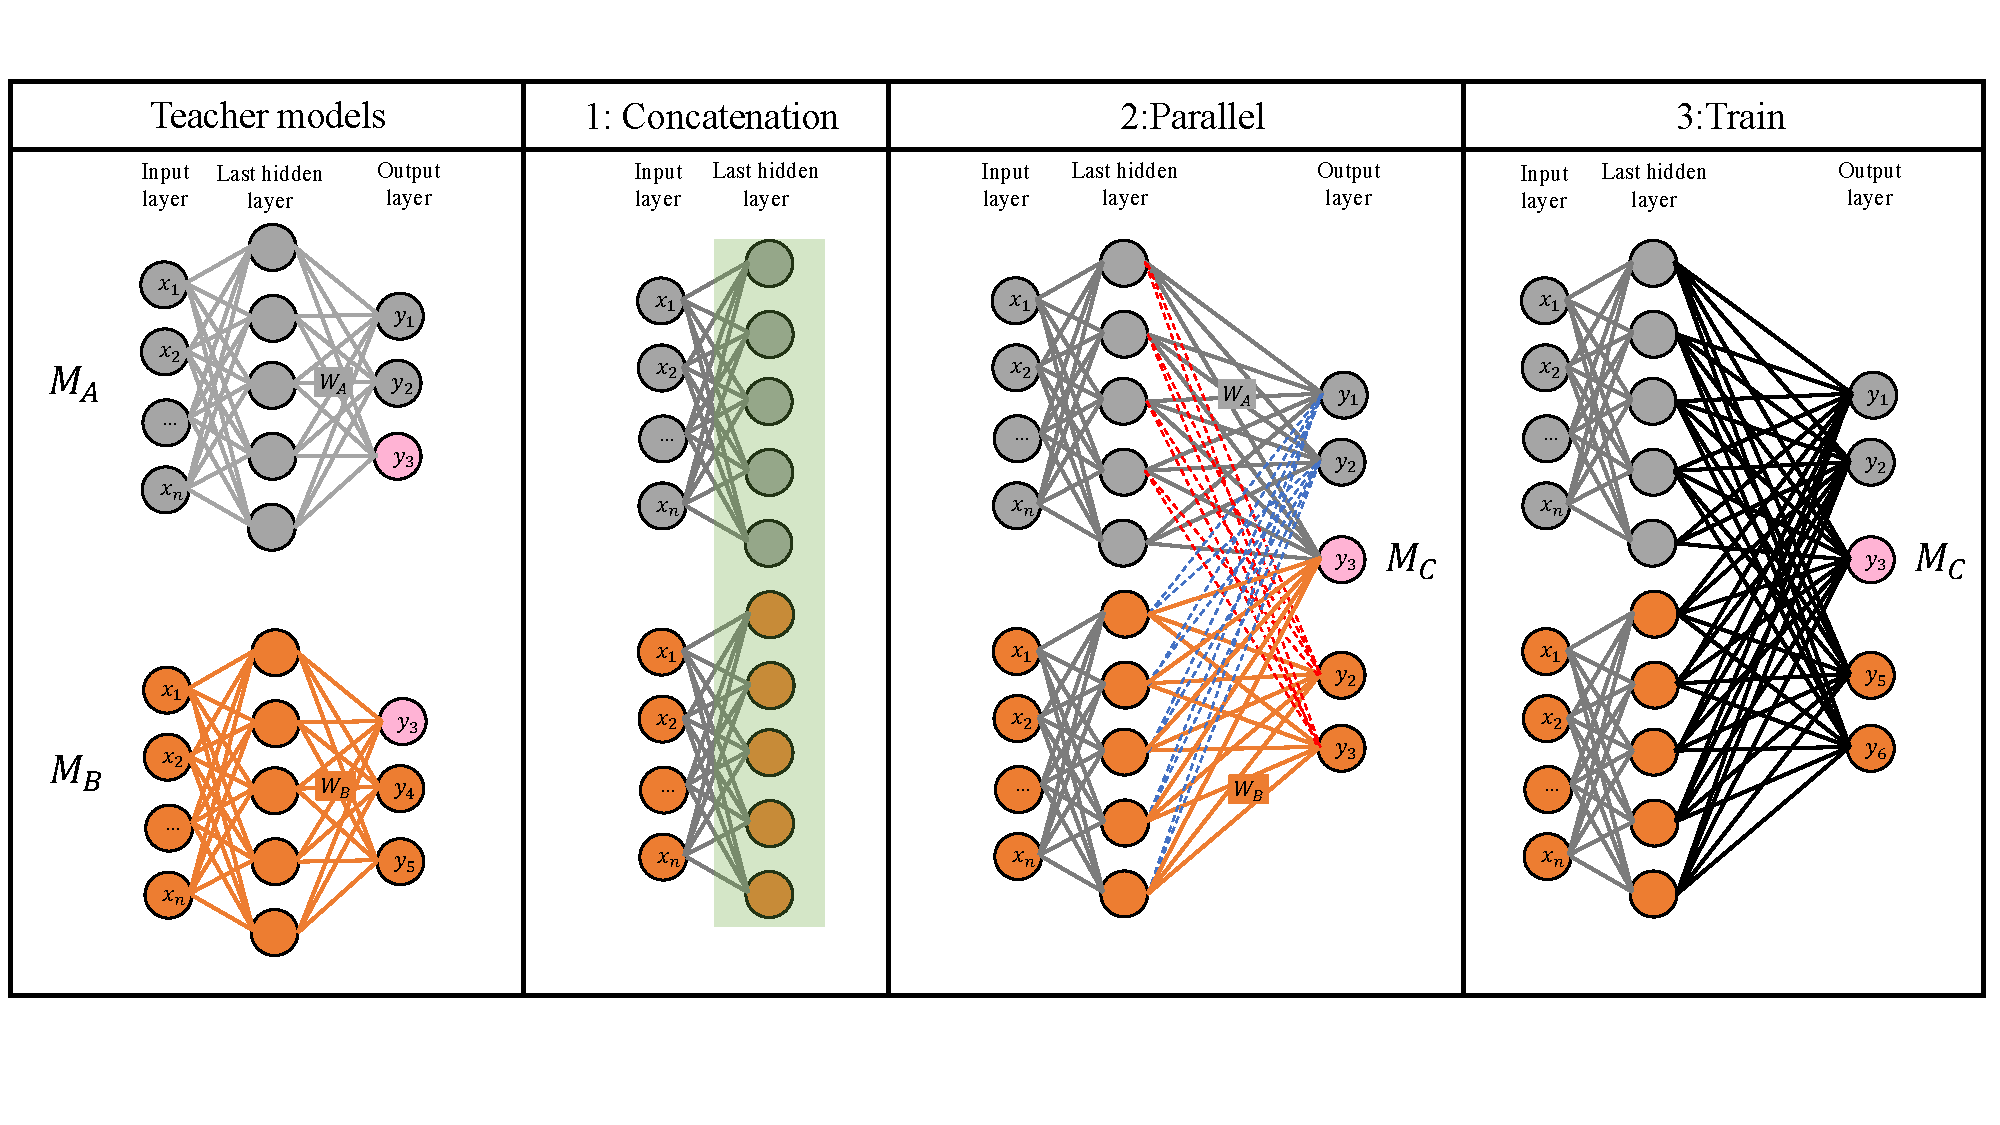
\includegraphics[scale=0.4]{MCCP_method.pdf}
	\caption{我们的MCCP方法的流程图。$\mathcal{W_A}$和$\mathcal{W_B}$分别表示最后一层$\mathcal{M_A}$和$\mathcal{M_B}$的权重。 绿色阴影层代表最后一个隐藏层的组合。 虚线的权重值为 0。}	
	\label{MCCP_method}
\end{figure}

\begin{equation}
	\label{weightFormula}
	\mathcal{W}_i = 
	\begin{cases}
		\hfil concat(\mathcal{W}_{i_\mathcal{A}},0) &  i \in unique_\mathcal{A} \;;\\
		\hfil concat(0,\mathcal{W}_{i_\mathcal{B}}) &  i \in unique_\mathcal{B} \;;\\
		concat(\mathcal{W}_{i_\mathcal{A}},\mathcal{W}_{i_\mathcal{B}}) &  i \in overlap \;.
	\end{cases}
\end{equation}

实验评估:

实验方法:我们引入了三种方法作为基线,包括 ICML’2019\cite{wu2019heterogeneous}的 HMR、IJCAI’2019\cite{luo2019knowledge}的 CFL)和一个通用基线(称为
Dummy)。 选择HMR和CFL的原因是这两种方法可以很好地迁移到我们的研究场景中。 即教师模型的训练集不可访问,教师模型可以是同构的,也可以是异构的。 Dummy是最直观的基线,它通过整合教师模型的输出来直接进行预测。

\begin{figure}[t]
	\subfigure[Car]{
		\begin{minipage}[b]{.3\linewidth}
			\centering
			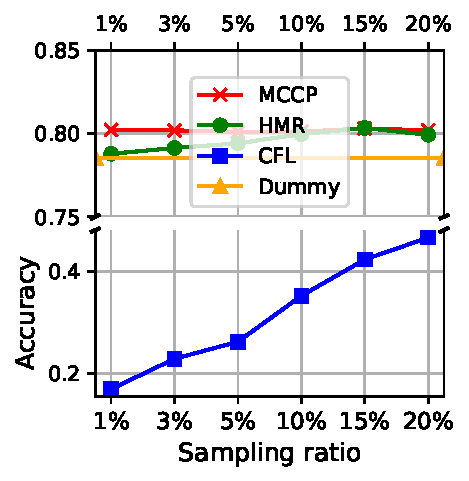
\includegraphics[scale=0.5]{./MCCP_results/car.pdf}
		\end{minipage}
	}
	\subfigure[Flower]{
		\begin{minipage}[b]{.3\linewidth}
			\centering
			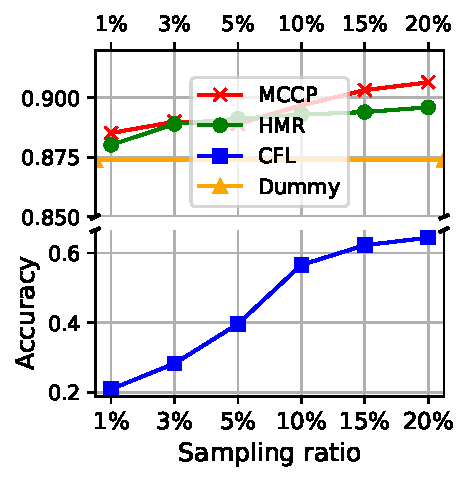
\includegraphics[scale=0.5]{./MCCP_results/flower.pdf}
		\end{minipage}
	}
	\subfigure[Food]{
		\begin{minipage}[b]{.3\linewidth}
			\centering
			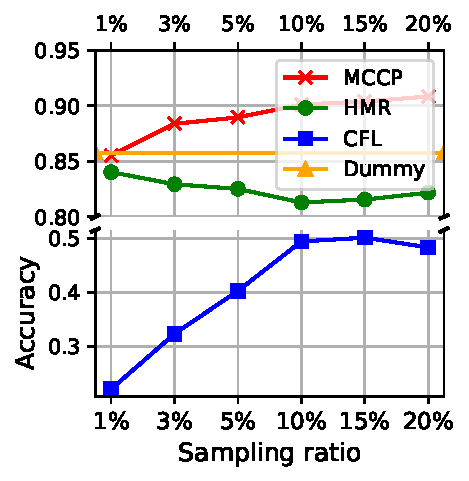
\includegraphics[scale=0.5]{./MCCP_results/food.pdf}
		\end{minipage}
	}
	
	\subfigure[Fruit]{
		\begin{minipage}[b]{.3\linewidth}
			\centering
			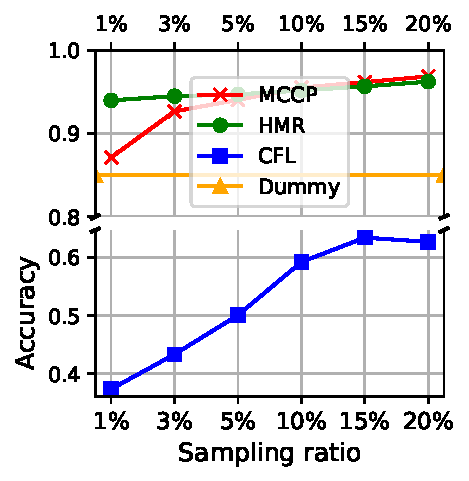
\includegraphics[scale=0.5]{./MCCP_results/fruit.pdf}
		\end{minipage}
	}
	\subfigure[Sport]{
		\begin{minipage}[b]{.3\linewidth}
			\centering
			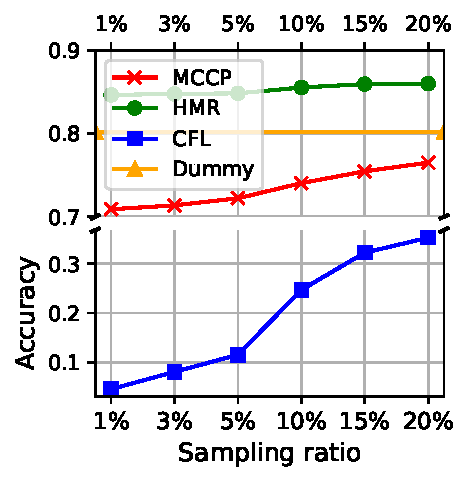
\includegraphics[scale=0.5]{./MCCP_results/sport.pdf}
		\end{minipage}
	}
	\subfigure[Weather]{
		\begin{minipage}[b]{.3\linewidth}
			\centering
			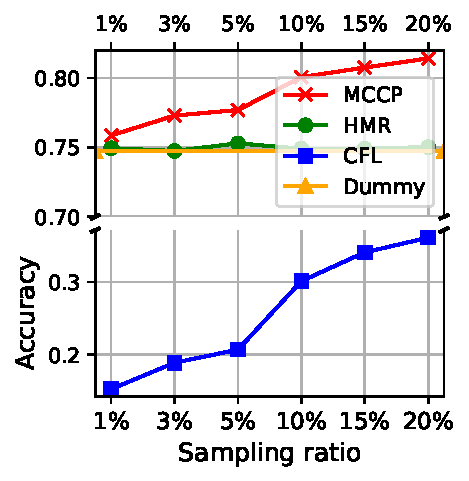
\includegraphics[scale=0.5]{./MCCP_results/weather.pdf}
		\end{minipage}
	}
	
	\subfigure[Animal\_1]{
		\begin{minipage}[b]{.3\linewidth}
			\centering
			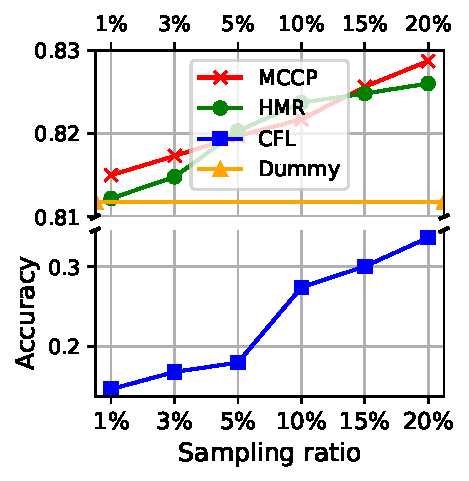
\includegraphics[scale=0.5]{./MCCP_results/animal_1.pdf}
		\end{minipage}
	}
	\subfigure[Animal\_2]{
		\begin{minipage}[b]{.3\linewidth}
			\centering
			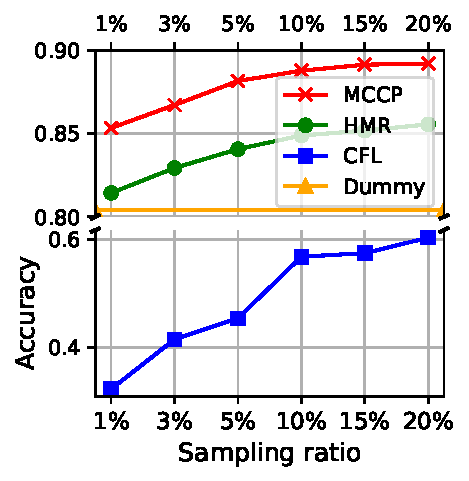
\includegraphics[scale=0.5]{./MCCP_results/animal_2.pdf}
		\end{minipage}
	}
	\subfigure[Animal\_3]{
		\begin{minipage}[b]{.3\linewidth}
			\centering
			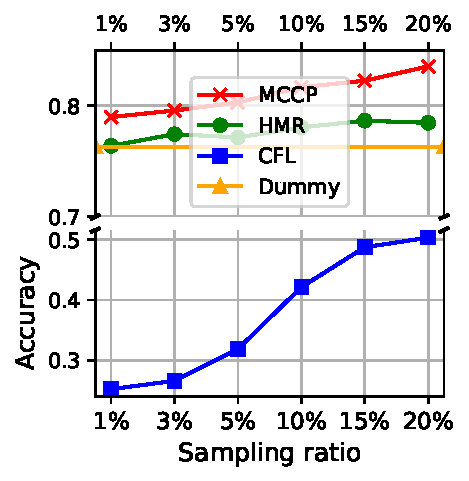
\includegraphics[scale=0.5]{./MCCP_results/animal_3.pdf}
		\end{minipage}
	}
	\caption{训练后学生模型的准确性。横轴表示用于训练的手动标注的采样比例,纵轴表示学生模型在混合测试集中的分类准确率。}
	\label{major_results}
\end{figure}

我们的实验可以分为两个步骤。 第一步是从混合测试集中采样以进行模型训练。采用随机抽样策略进行抽样,抽样比例为1\%、3\%、5\%、10\%、15\%、20\%\cite{shen2020multiple}。 第二步是训练学生模型,训练轮数为5。在混合测试集上评估学生模型的分类精度。

实验结果:实验结果如图\ref{major_results}所示。每个子图对应一个领域,横轴表示采样比例,纵轴表示学生模型在混合测试集上的分类精度。 Dummy方法是一条横线,因为Dummy方法没有训练过程,只使用教师模型置信度最高的标签作为预测标签。 从图中可以看出,随着训练样本数量的增加,模型的性能将会提高。 其中,CFL的性能提升最快,这是由于CFL的初始精度较低。 CFL在训练前没有结合教师模型,而是使用新的未经训练的模型作为学生模型。只是在后续的训练过程中,通过知识蒸馏的方法将教师模型的判别能力蒸馏到学生模型中。 因此,CFL方法的学生模型在训练之前并没有重用教师模型的知识。综合来看,可以看出,在大多数情况下,9个领域中的8个,MCCP 的性能都优于其他方法,而 CFL 的准确率最低,但其性能提升最快。

\begin{framed}
	\noindent 实验发现MCCP在训练后在混合测试集上表现更好,在大多数情况下超过了基线。(已投稿至JSME期刊并获得审稿人的major revision意见)
\end{framed}




\subsection{基于熵的木马输入检测技术}

随着将传统软件测试中的变异测试\cite{jia2010analysis}引入到深度学习软件\cite{shen2018munn,ma2018deepmutation}之后,深度学习变异测试已广泛应用于许多新的场景中。变异测试的核心技术是变异算子。Ma等\cite{ma2018deepmutation}提出的DeepMutation涵盖了16种(8种代码级和8种模型级)深度学习变异算子。在后门攻击场景下,代码级的变异操作是不适用的,因为我们仅仅只能访问被植入后门的模型,没有训练集和训练代码。Wang等\cite{wang2019adversarial}应用深度学习变异测试去检测对抗样本,他们的核心观察是对抗样本往往更接近决策边界,这使得利用变异技术来检测对抗样本成为可能。

与Wang\cite{wang2019adversarial}等提出的视角相反,我们假设木马样本对模型的决策边界并不敏感。我们提出了基于熵的木马输入检测ETID(Entropy-Based Trojaned InputDetection)该方法大体上分成两部分,第一步先确定哪一个分类是攻击的目标分类;第二步再根据模型的预测信息的熵来确定某一个输入样本是不是木马样本。我们的方法结合了两种思想:

\begin{itemize}
	\item 决策边界\cite{shen2020mcp}:通过变异操作对被植入后门的模型进行变异,改变模型的决策边界,通过计算各个分类子集在决策边界的改变精度,根据我们的假设,精度越高越有可能是攻击目标类别。
	\item 预测信息熵\cite{gao2019strip}:在确定攻击类别后,我们根据一个输入在不同变异模型上输出的结果,计算该样本的预测熵。因此有很高的概率变异模型对后门样本的检测功能不变,但是对普通干净样本而言,变异模型对其预测标记会发生改变。而且由于我们的变异操作是随机不可控的,所以不同的变异输出类别很可能是不同的。也就是样本的熵会比较大,同时后门样本的熵会比较小甚至接近于0,因为针对某个后门样本每一个变异模型的输出类别都是一样的。因此根据信息熵就可以检测出某个输入样本是否是木马输入样本。
\end{itemize}

\begin{figure}[h]
	\centering
	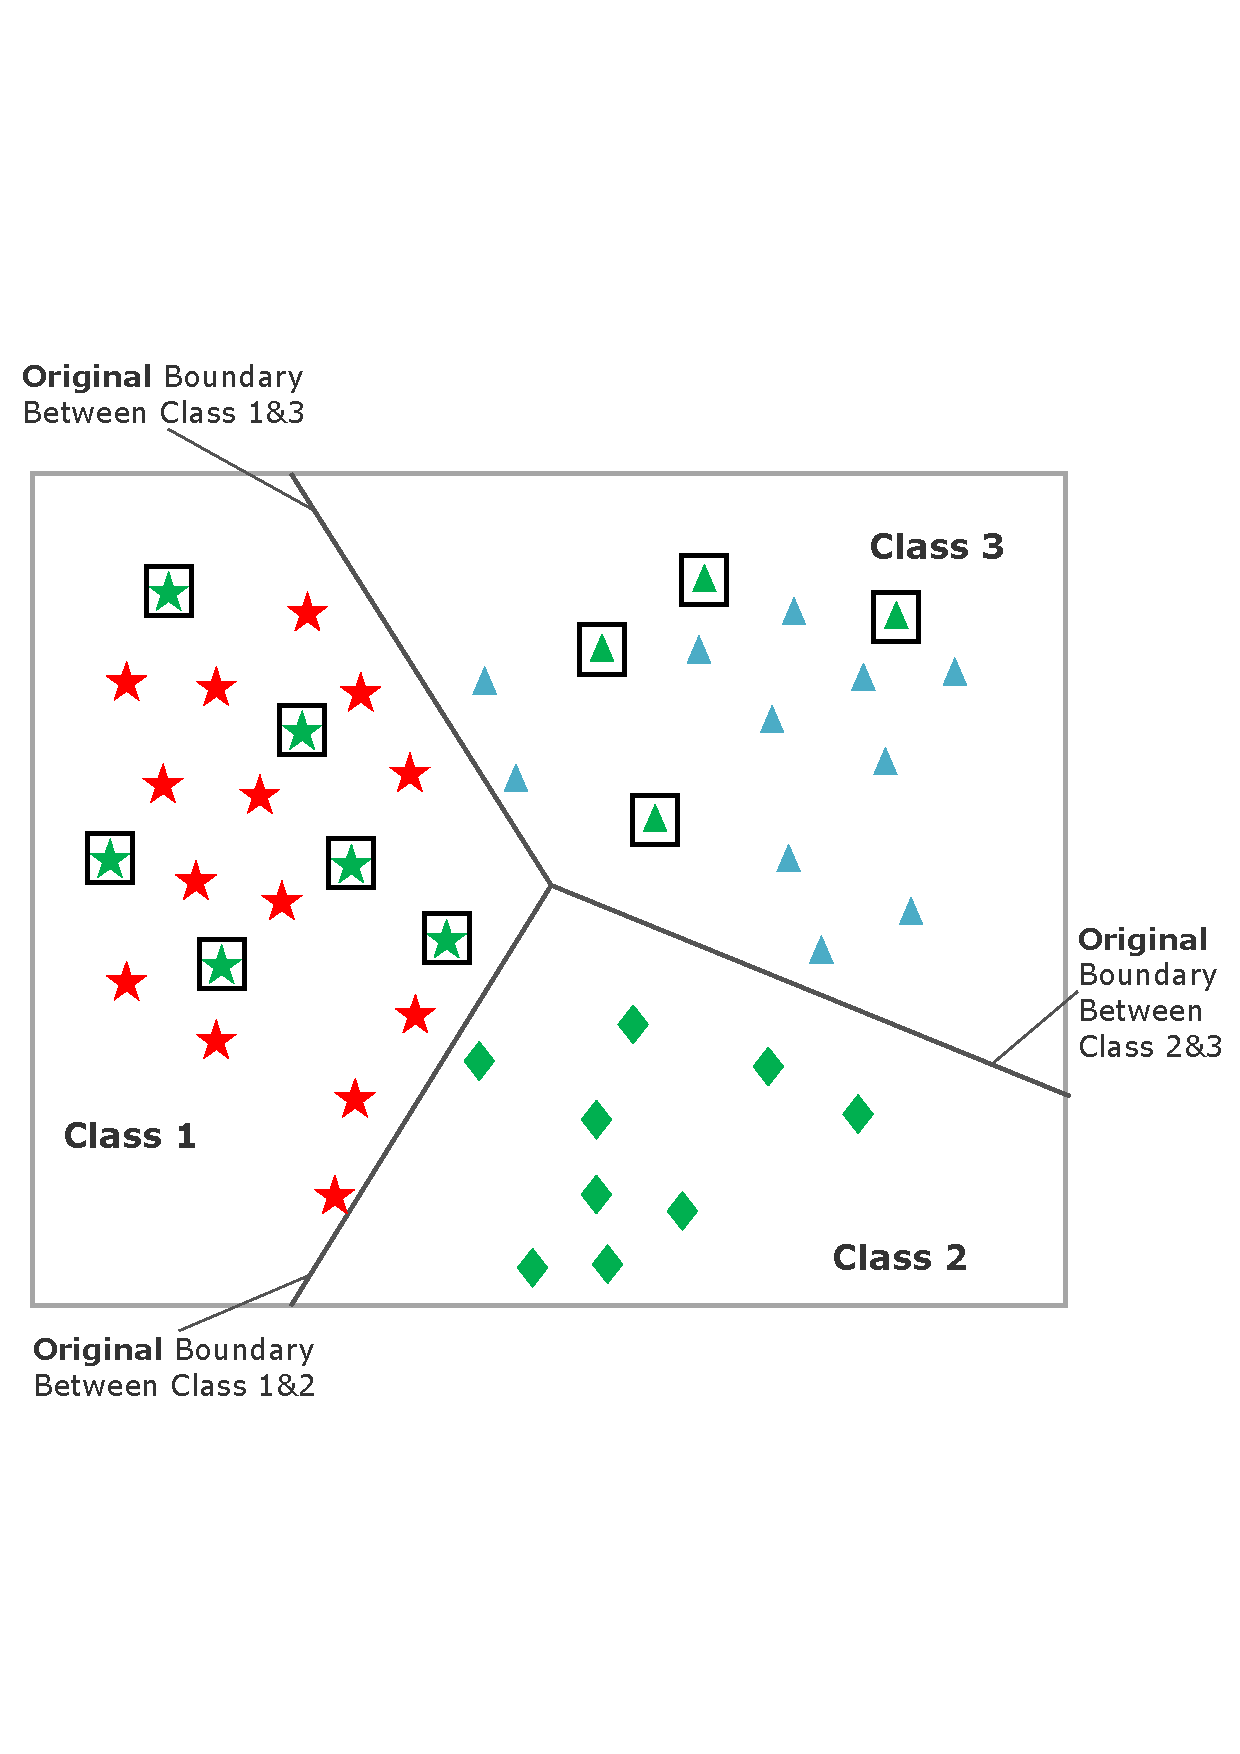
\includegraphics[width=0.48\linewidth]{Backdoor.pdf}
	\caption{一个被植入后门的多分类深度学习模型 $\mathcal{M}_\mathcal{I}$}
	\label{Backdoor_injected_model}
\end{figure}

图\ref{Backdoor_injected_model}展示了一个被注入后门的多分类模型$\mathcal{M}_\mathcal{I}$的例子。具体来看该模型是一个三分类模型,类别 1: $\bigstar$, 类别 2: $\blacklozenge$, 和类别3 $\blacktriangle$。这些样本被原始模型 $\mathcal{M}_\mathcal{O}$自带的原始边界(实线)分成了三类。不带框的形状($\bigstar$,$\blacklozenge$,$\blacktriangle$)代表普通干净样本,颜色(红,绿,蓝)代表被$\mathcal{M}_\mathcal{I}$预测的结果,框子表明木马样本。正如图\ref{Backdoor_injected_model}所看到的干净的样本都被$\mathcal{M}_\mathcal{I}$正确分类了,但是被攻击者注入后门的带框样本都被$\mathcal{M}_\mathcal{I}$分类成了类别2。综上所述,我们获得了以下观察发现:

1)木马样本与原始的模型的决策边界没有明显的关系,即这些样本与普通干净的样本相比并没有更接近决策边界。

2)深度神经网络模型被变异后,其决策边界发生改变。木马样本没有很高的概率跨越改变后的决策边界,因此这些样本的预测结果可能保持不变。

3)攻击者设计的后门触发是隐蔽的(很难去被察觉)同时也很难去消除。


方法介绍:

生成变异模型:
变异算子是变异测试的核心技术,用于变异原始深度学习模型。 最近,Shen等人提出了一种称为 MuNN\cite{shen2018munn} 的深度学习突变方法,由 5 个模型级突变算子组成,用深度学系突变体。之后,Ma等人提出了一种更全面的深度学习变异技术,称为DeepMutation\cite{ma2018deepmutation},它包含16个(即8个源级和8个模型级)深度学习变异算子。 在后门攻击场景中,源级变异算子不适合,因为我们只能获取后门注入的深度学习模型,而不能获取训练数据或训练代码。 具体来说,在本研究中,我们在 DeepMutation\cite{ma2018deepmutation}中采用了 5 个模型级 深度学习特定变异算子如下表\ref{Mutation_Operator}所示,它们在语法上与 MuNN\cite{shen2018munn}中的变异算子相似。 没有考虑算子“Layer Deactivation(M)”和“Layer Addition(M)”,因为我们研究的深度学习模型不满足结构条件。 此外,我们进一步删除了算子“Activation Function Removal(M)”,因为该算子只能生成很少数量的突变体(与深度学习模型中的层数一致),这不适合我们的工作。
\newcommand{\tabincell}[2]{
	\begin{tabular}{@{}#1@{}}#2
	\end{tabular}
}  %表格自动换行


\begin{table}[t] 
	\centering
	\caption{采用的5种模型级变异算子}
	%  \vspace{2ex}
	\label{Mutation_Operator}
	\begin{threeparttable}
		\begin{tabular}{lll}
			\toprule
			变异算子 & 级别 & 详情\\
			\midrule
			Gaussian Fuzzing&Weight& \tabincell{c}{Fuzz weight by \\Gaussian Distribution}  \\	
			\midrule
			Weight Shuffling& Neuron& \tabincell{c}{Shuffle weights \\of selected neurons} \\	
			\midrule
			\tabincell{c}{ Neuron Effect Blocking} & Neuron&Block selected neurons \\	
			\midrule
			\tabincell{c}{Neuron Activation Inverse} &Neuron & \tabincell{c}{Reverse the activation \\of selected neurons} \\	
			\midrule
			Neuron Switch& Neuron& \tabincell{c}{Switch two selected \\ neurons in one layer} \\		
			\bottomrule
		\end{tabular}
	\end{threeparttable}
\end{table} 

第一步:确定攻击分类:

我们在实验中观察到一个现象:注入后门的深度学习模型对于目标(受攻击)类别的突变非常稳健,可用于在检测中首先识别目标类别。 在在线后门检测之前,我们借助三个研究数据集的测试集 T 来识别目标类别,即 MNIST、CIFAR10 和 GTSRB,其大小分别为 10,000、10,000 和 12,630。
首先,我们计算了每个突变体在每个类别的原始训练集 $\mathcal{T}$ 上的准确性。 例如,对于类别$\mathcal{c}$,我们首先选择$\mathcal{T}$ 中真实标签为$\mathcal{c}$的所有测试样本组成子集$\mathcal{T}_c$。$c$类在突变体、$\mathcal{M}_m$上的准确率为$\mathcal{ACC(M}_c,\mathcal{T}_c)$。变异模型的变异率从1\%,3\%,5\%,10\%,20\%,30\%,40\%,50\%,60\%,70\%,80\%逐渐增加,直到精度的平均值和中位值均为最大的分类上的精度分布与其他类有显著性差异,则停止变异,确定当前变异率为所有变异算子的变异率,该类别为目标类别。显然,对于每个数据集和攻击场景,我们可以在每个输出类别中获得 250 个变异精度值

第二步:检测后门样本:

变异模型排序:
首先,人工从攻击类别中选择少量干净样本。计算变异模型在干净样本和剩余样本的精度差。差值越小的变异模型优先级越高,以此对变异模型进行排序。

具体来说,例如,如果在第一步中确定攻击目标类为类1,我们就人工从类别为1的样本中,选择少量的干净样本作为干净种子集合记为$Seed_{clean}$,则类1中剩余的样本集合记为$RemainSet$。然后计算变异模型$\mathcal{M}_m$在$Seed_{clean}$上的准确度,记为$\mathcal{ACC(}\mathcal{M}_m, Seed_clean\mathcal{)}$,  计算变异模型$\mathcal{M}_m$在$RemainSet$上的准确度,记为$\mathcal{ACC(}\mathcal{M}_m, RemainSet\mathcal{)}$。用$\mathcal{ACC(}\mathcal{M}_m,Seed_clean\mathcal{)}-\mathcal{ACC(}\mathcal{M}_m,RemainSet\mathcal{)}$表示变异模型$\mathcal{M}_m$的优先级值,值越小则优先级越高,以此优先级生成变异模型的优先级队列。

基于熵的后门检测:
选择前50的变异模型,在攻击目标类中计算样本的预测分类结果的熵。熵越大则该样本越可能为后门样本。

具体来说,紧接上一步,我们从变异模型优先级队列中取出前50个变异模型作为我们变异模型组。将攻击目标类(如类别1)中的每个样本都喂给每个变异模型,即获得每个待测样的50个预测标签列表,进而计算每个预测标签列表的信息熵。根据我们的见解,干净样本对模型的变异更为敏感,故熵越大则该样本越可能为后门样本。将熵值作为优先级,我们可以获得待测样本的优先级队列(即越靠近队头越有可能为后门样本)。

具体的实现算法如\ref{algo_BSD}所示


\begin{algorithm}
	\caption{Backdoor Sample Detection}
	\label{algo_BSD}
	\SetKwData{mutationRate}{mutationRate}\SetKwData{mutationRateList}{mutationRateList}\SetKwData{mutationModelList}{mutationModelList}\SetKwData{targetClass}{targetClass}\SetKwData{adaptiveRate}{adaptiveRate}
	\SetKwData{seedSet}{seedSet}\SetKwData{remainSet}{remainSet}\SetKwData{mutationModel}{mutationModel}
	\SetKwData{accSeed}{accSeed}\SetKwData{accRemain}{accRemain}
	\SetKwData{mutationModelQueue}{mutationModelQueue}
	\SetKwData{priority}{priority}\SetKwData{targetClassSet}{targetClassSet}
	\SetKwData{selectedMutaionModels}{selectedMutaionModels}\SetKwData{sample}{sample}\SetKwData{entropy}{entropy}
	\SetKwFunction{Union}{Union}\SetKwFunction{FindCompress}{FindCompress}
	\SetKwFunction{genMutationModels}{genMutationModels}
	\SetKwFunction{getTargetClass}{getTargetClass}
	\SetKwFunction{getTargetClassSet}{getTargetClassSet}
	\SetKwFunction{selectSeed}{selectSeed}
	\SetKwFunction{calculateEntropy}{calculateEntropy}
	
	\KwIn{Poisoned dataset $D$, Backdoor model $M$}
	\KwOut{Sample Priority Queue $Q$}
	\BlankLine
	\mutationRateList $\leftarrow$ [1\%,3\%,5\%,10\%,20\%,30\%,40\%,50\%,60\%,70\%,80\%]\;
	\targetClass $\leftarrow$ $-1$\;
	\tcp{\textcolor{red}{The First step:Getting adaptive mutation rates and attacking target classes}}
	\mutationModelList $\leftarrow$ None\;
	\For{\mutationRate $\in$ \mutationRateList}{
		\mutationModelList $\leftarrow$ \genMutationModels{$M$,\mutationRate}\;
		\targetClass $\leftarrow$ \getTargetClass{$D$, \mutationModelList }\;
		\If{\targetClass $\neq -1$}{
			\mutationModelList = \mutationModelList\;
			\targetClass = \targetClass\;
			break\;
		}
	}
	\tcp{\textcolor{red}{Selecting clean sample seeds from the attack target class}}
	\targetClassSet $\leftarrow$ \getTargetClassSet{$D$,\targetClass}\;
	\seedSet, \remainSet $\leftarrow$ \selectSeed{\targetClassSet}\;
	\tcp{\textcolor{red}{Ranking the mutaion models}}
	\mutationModelQueue $\leftarrow$ PriorityQueue()\;
	\For{\mutationModel $\in$  \mutationModelList}{
		\accSeed $\leftarrow$ \mutationModel.eval(\seedSet)\;
		\accRemain $\leftarrow$ \mutationModel.eval(\remainSet)\;
		\priority $\leftarrow$ \accSeed-\accRemain\;
		\mutationModelQueue.put(\priority, \mutationModel)\;
	}
	\tcp{\textcolor{red}{Selection of top 50 mutation models}}
	\selectedMutaionModels $\leftarrow$ \mutationModelQueue.getTop50()\;
	\tcp{\textcolor{red}{The Second step:Calculate the entropy of the samples in the target class of the attack on the mutation model}}
	$Q$ $\leftarrow$ PriorityQueue()\;
	\For{\sample $in$ \targetClassSet}{
		\entropy $\leftarrow$ \calculateEntropy{\sample,\selectedMutaionModels}\;
		$Q$.put(\entropy, \sample)\;
	}
	return $Q$\;
	
\end{algorithm}


我们在三个图像数据集(MINST、CIFAR-10、GTSRB)上进行了实验。其中第一步和第二步实验结果分布如图\ref{target_class}和图\ref{detect}所示,我们的方法在攻击类别的确定和后门样本的检测均取得了较好的效果。


\begin{figure}[t]
	\subfigure[Car]{
		\begin{minipage}[b]{.3\linewidth}
			\centering
			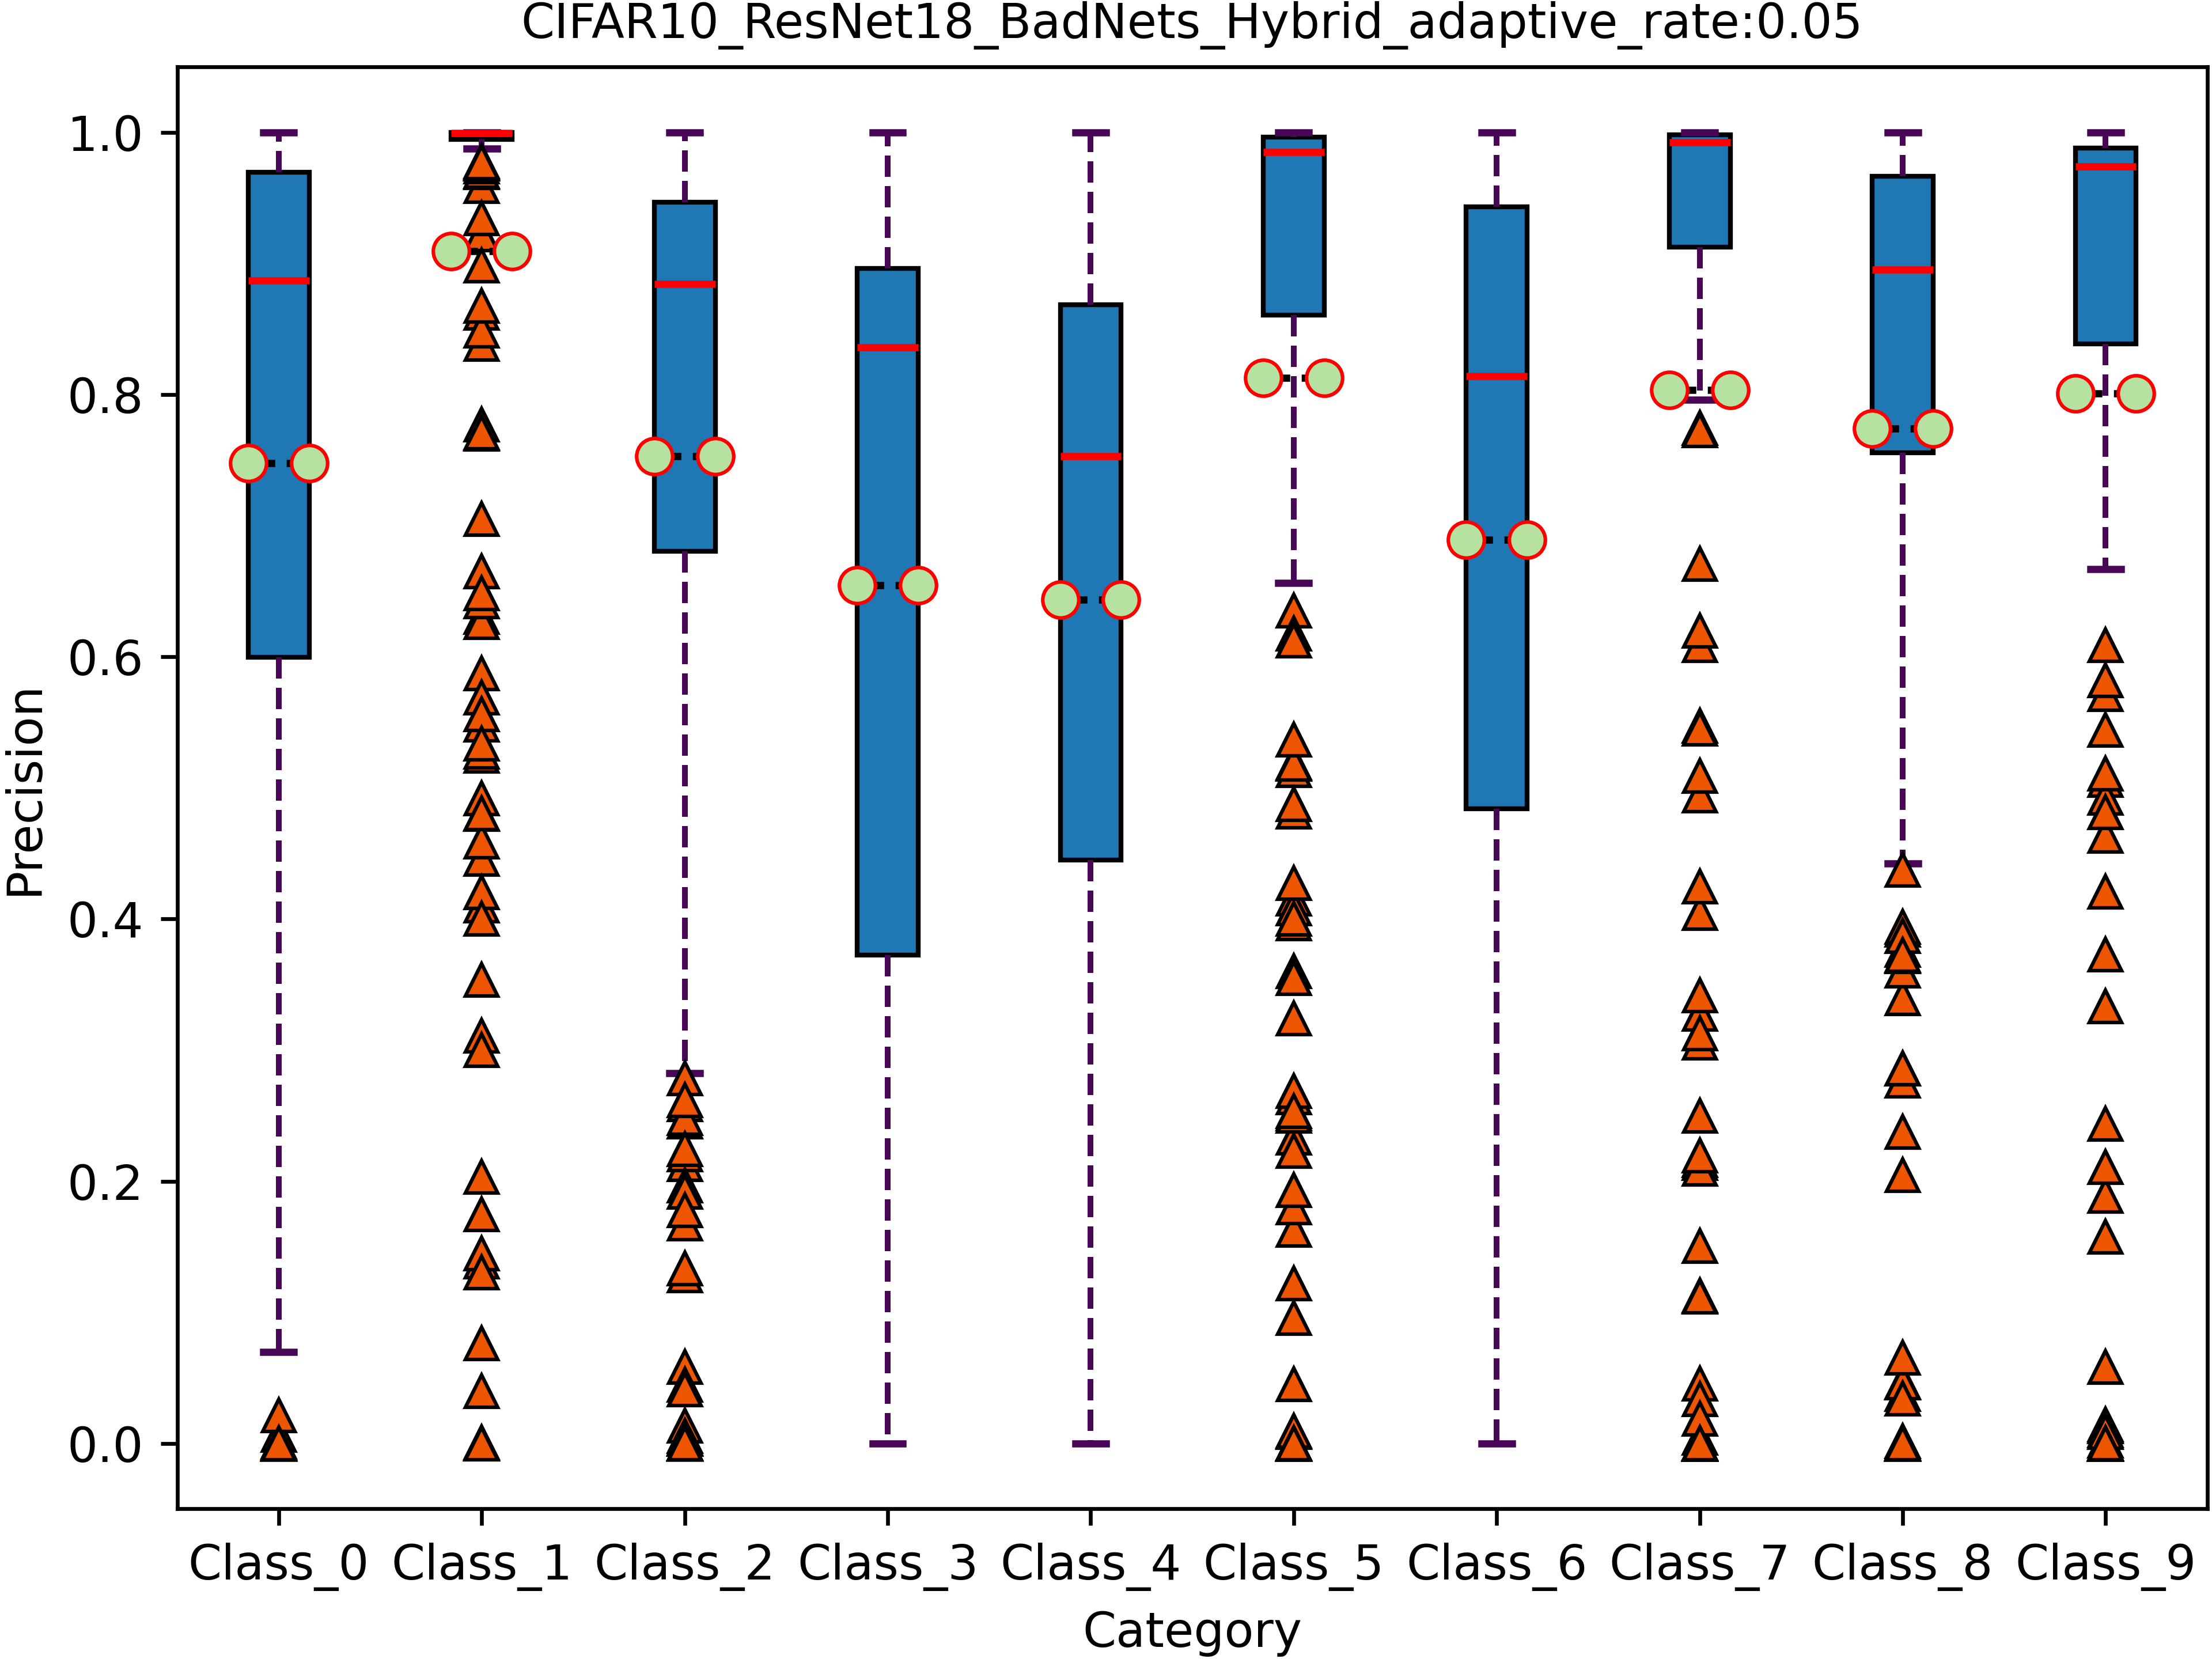
\includegraphics[scale=0.3]{./Backdoor_detect_result/target_class/BadNets.png}
		\end{minipage}
	}
	\subfigure[Flower]{
		\begin{minipage}[b]{.3\linewidth}
			\centering
			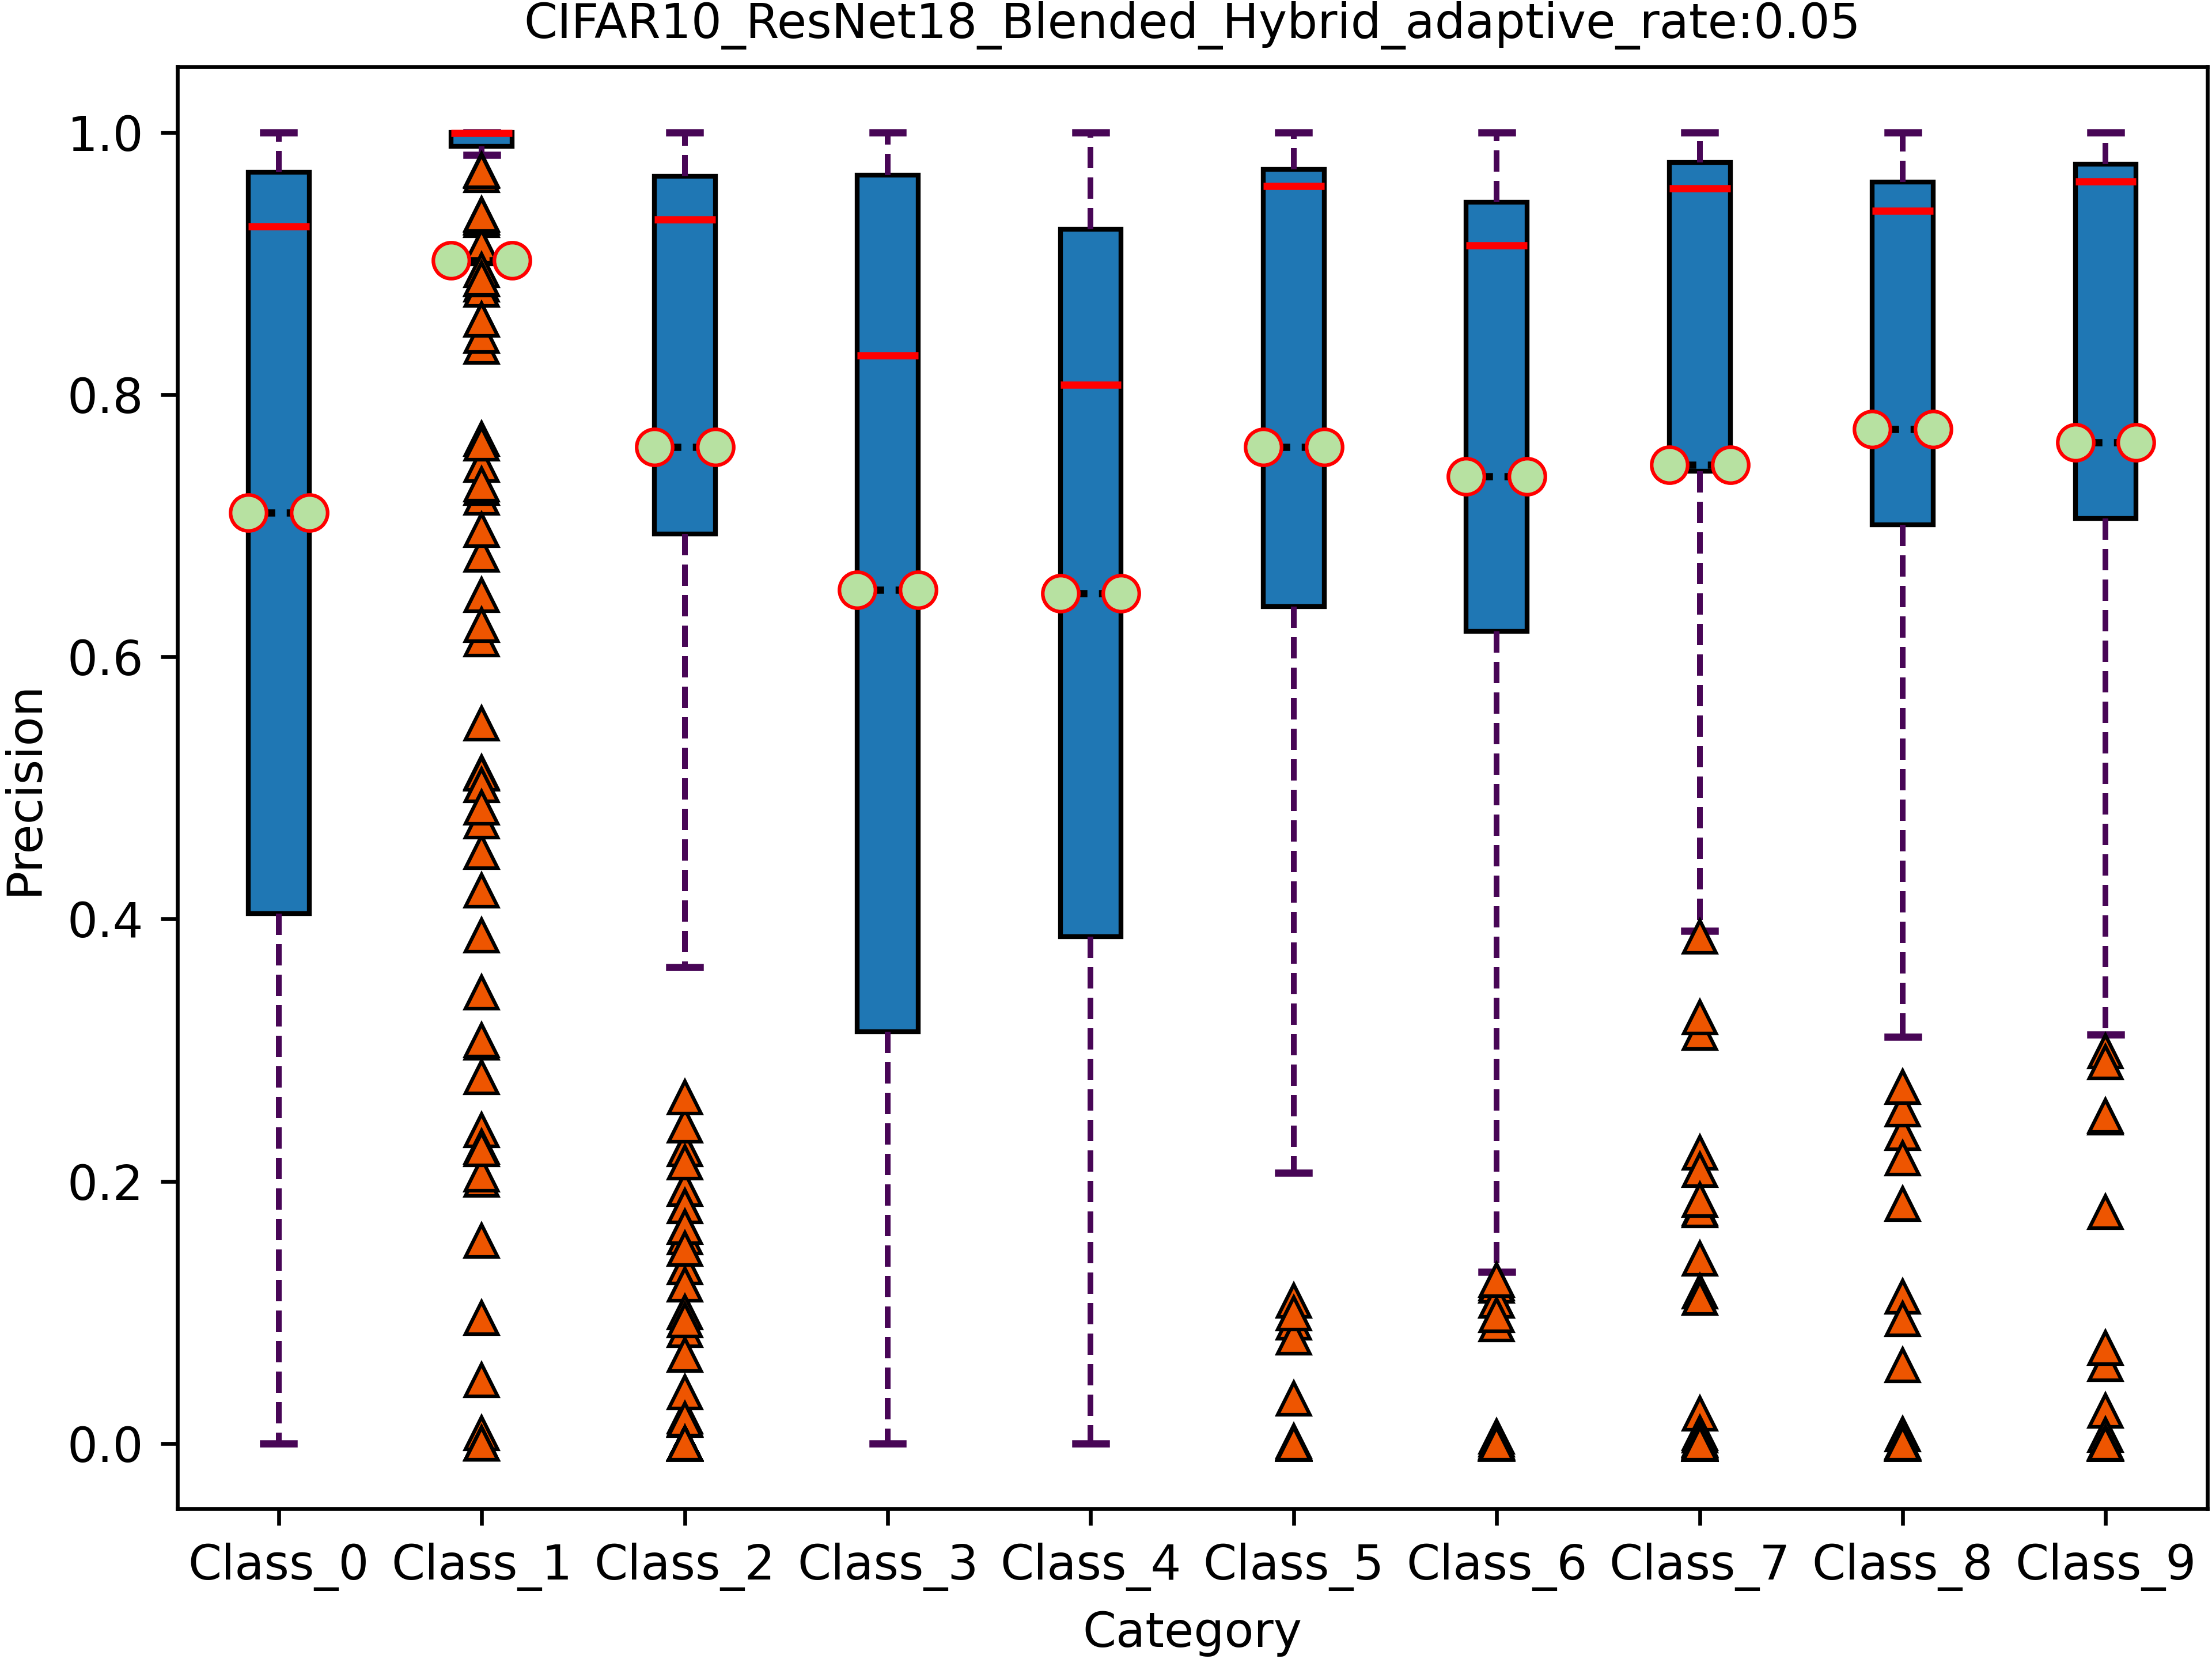
\includegraphics[scale=0.3]{./Backdoor_detect_result/target_class/Blended.png}
		\end{minipage}
	}
	\subfigure[Food]{
		\begin{minipage}[b]{.3\linewidth}
			\centering
			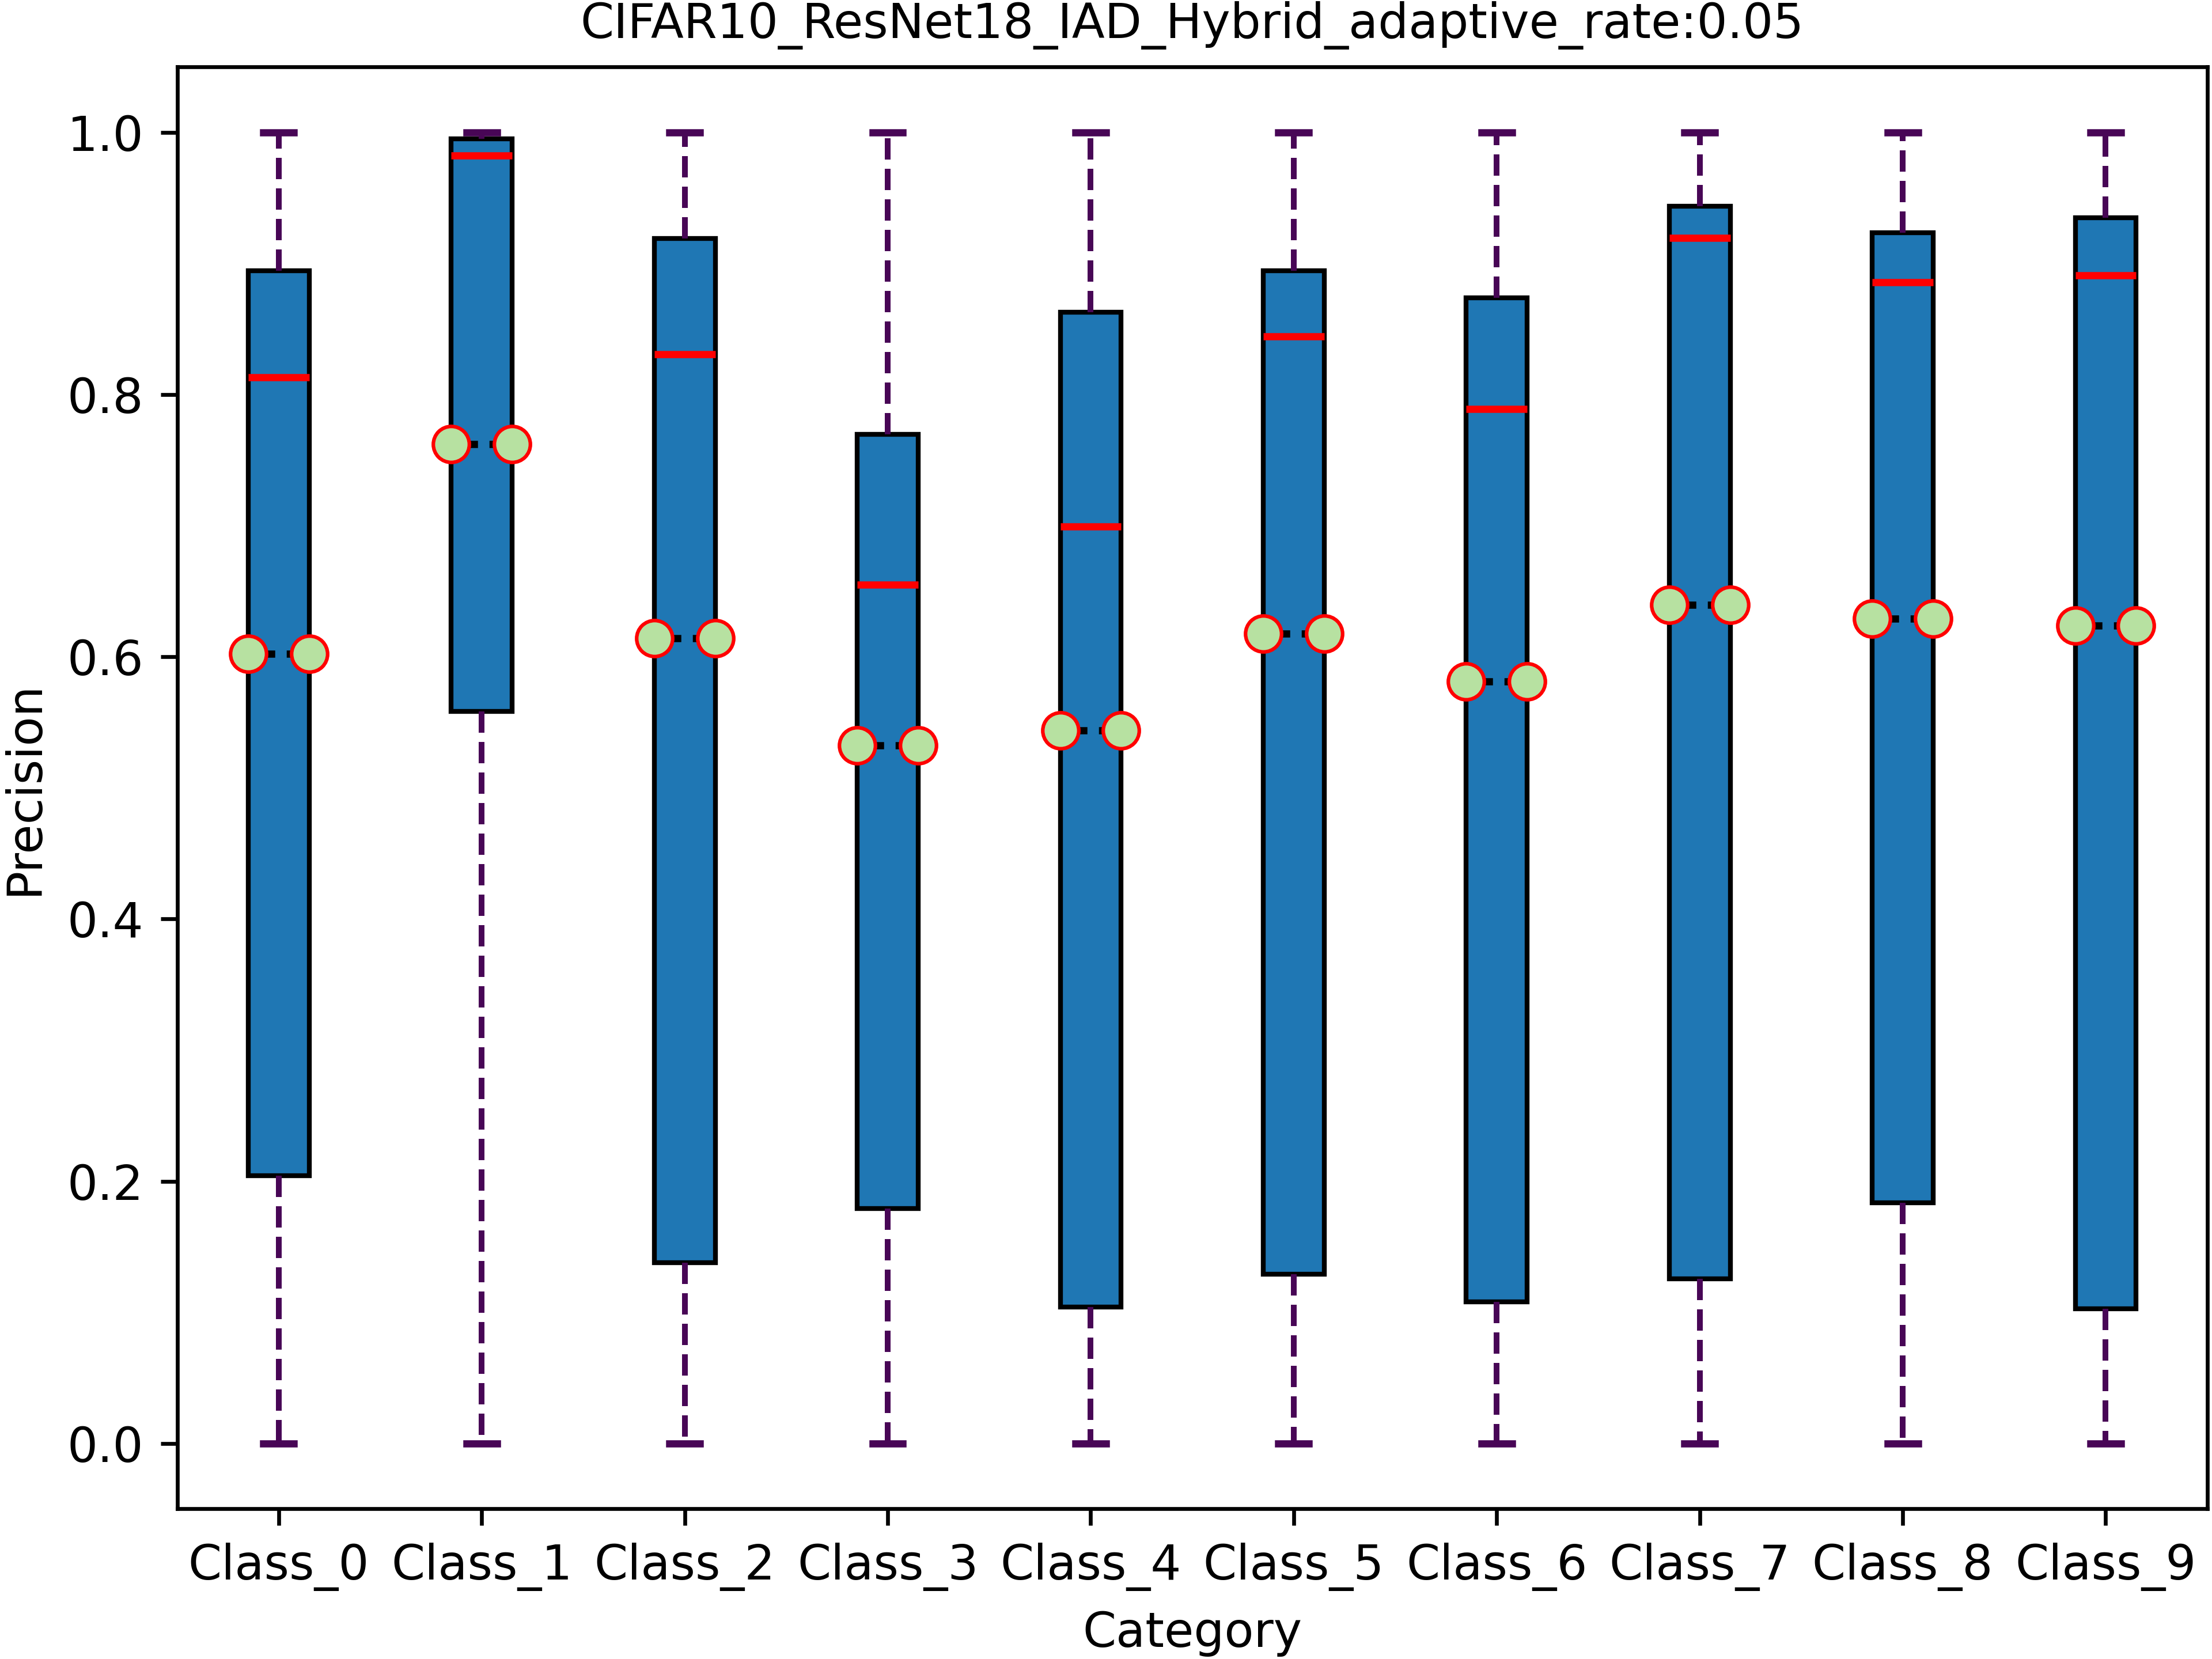
\includegraphics[scale=0.3]{./Backdoor_detect_result/target_class/IAD.png}
		\end{minipage}
	}
	
	\subfigure[Fruit]{
		\begin{minipage}[b]{.3\linewidth}
			\centering
			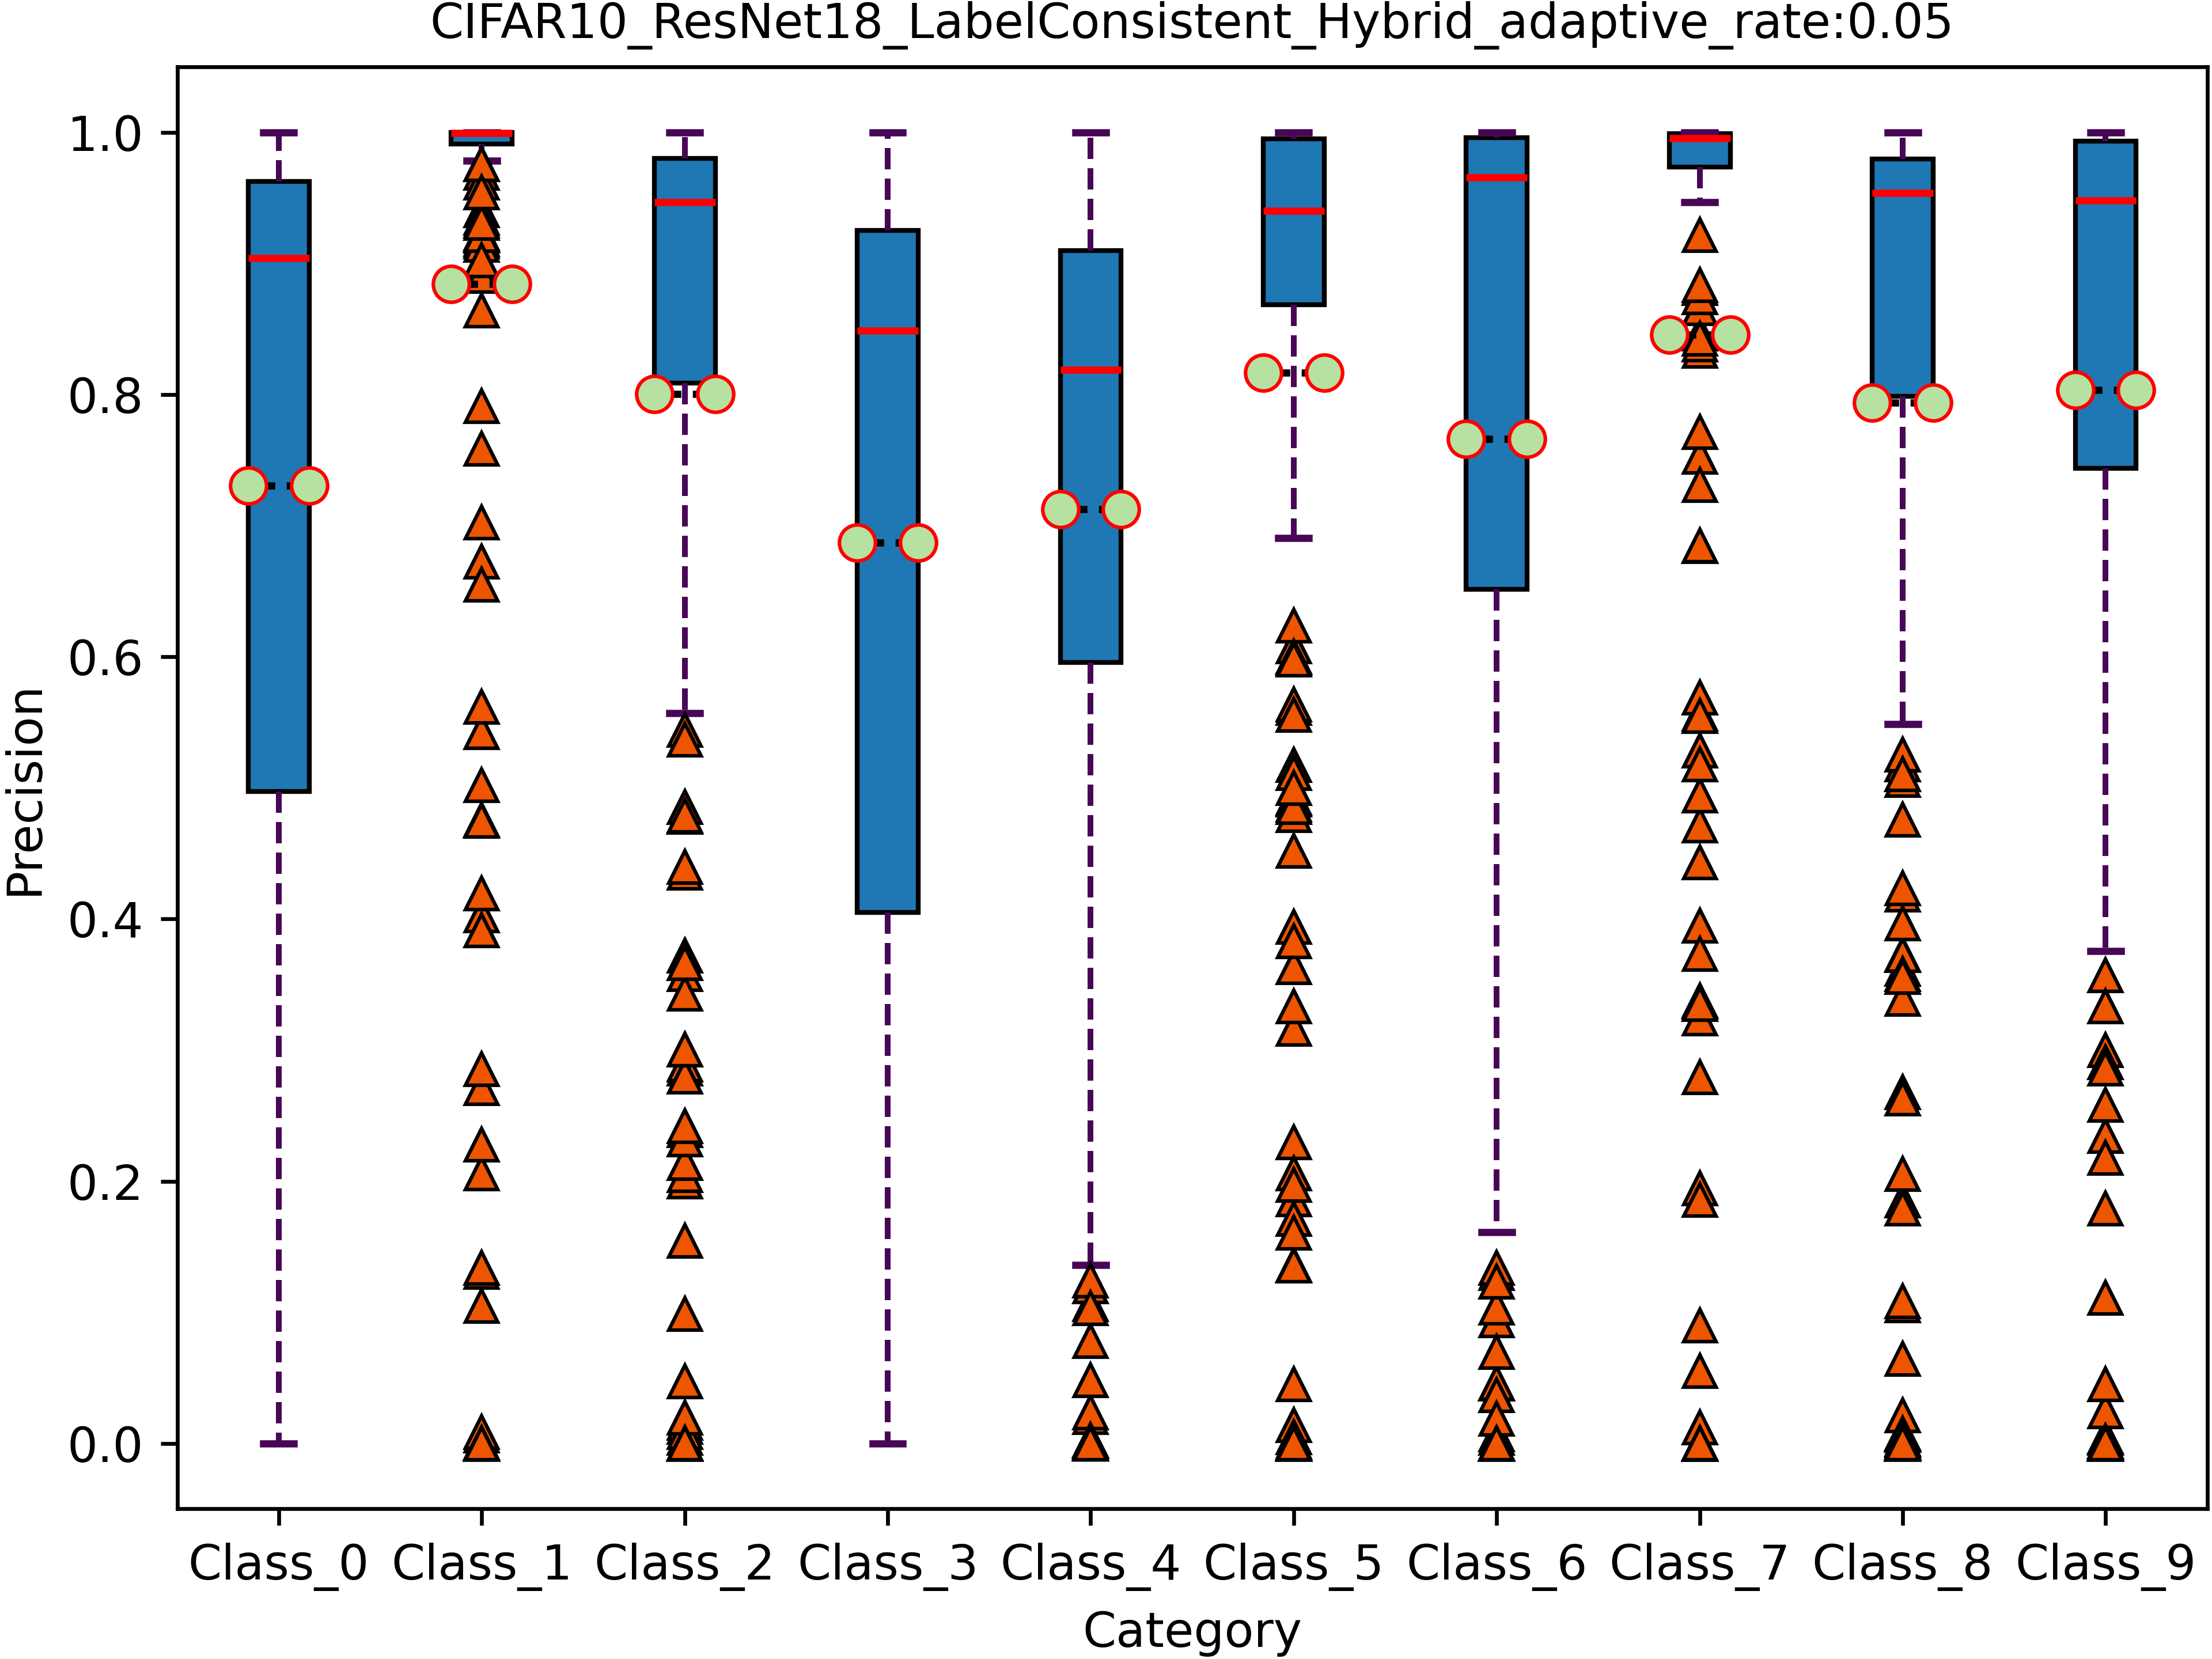
\includegraphics[scale=0.3]{./Backdoor_detect_result/target_class/LabelConsistent.png}
		\end{minipage}
	}
	\subfigure[Sport]{
		\begin{minipage}[b]{.3\linewidth}
			\centering
			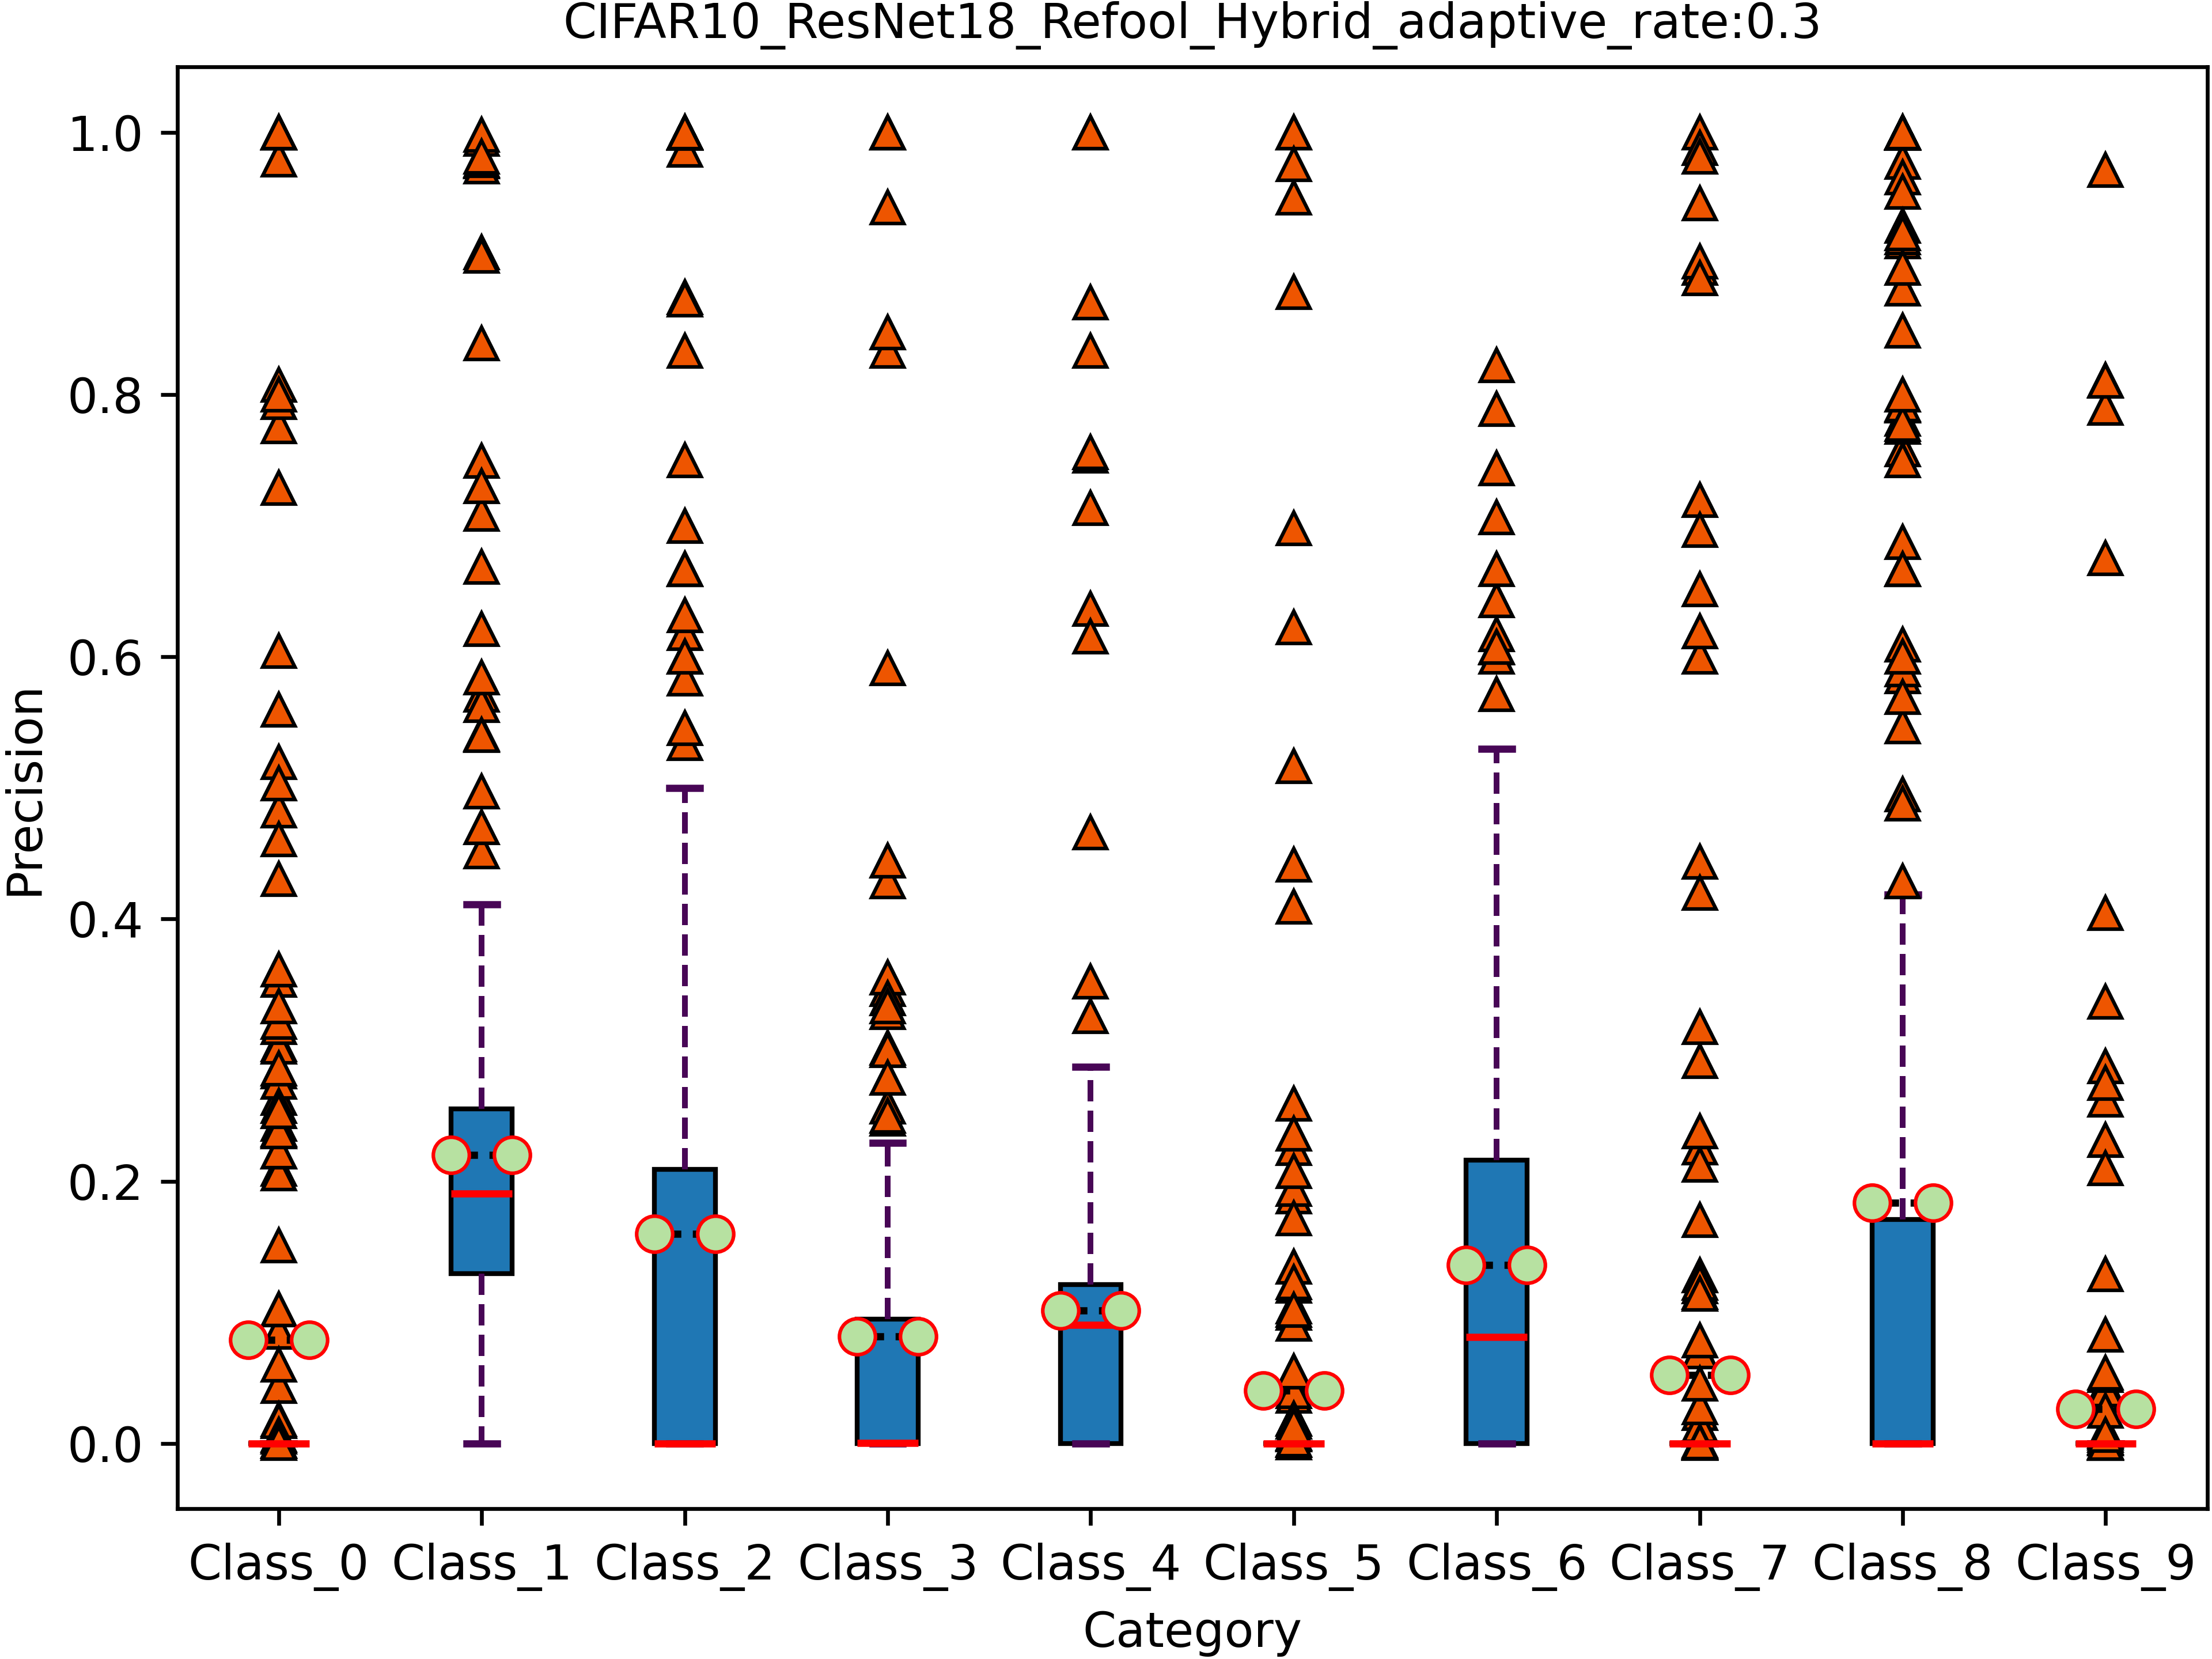
\includegraphics[scale=0.3]{./Backdoor_detect_result/target_class/Refool.png}
		\end{minipage}
	}
	\subfigure[Weather]{
		\begin{minipage}[b]{.3\linewidth}
			\centering
			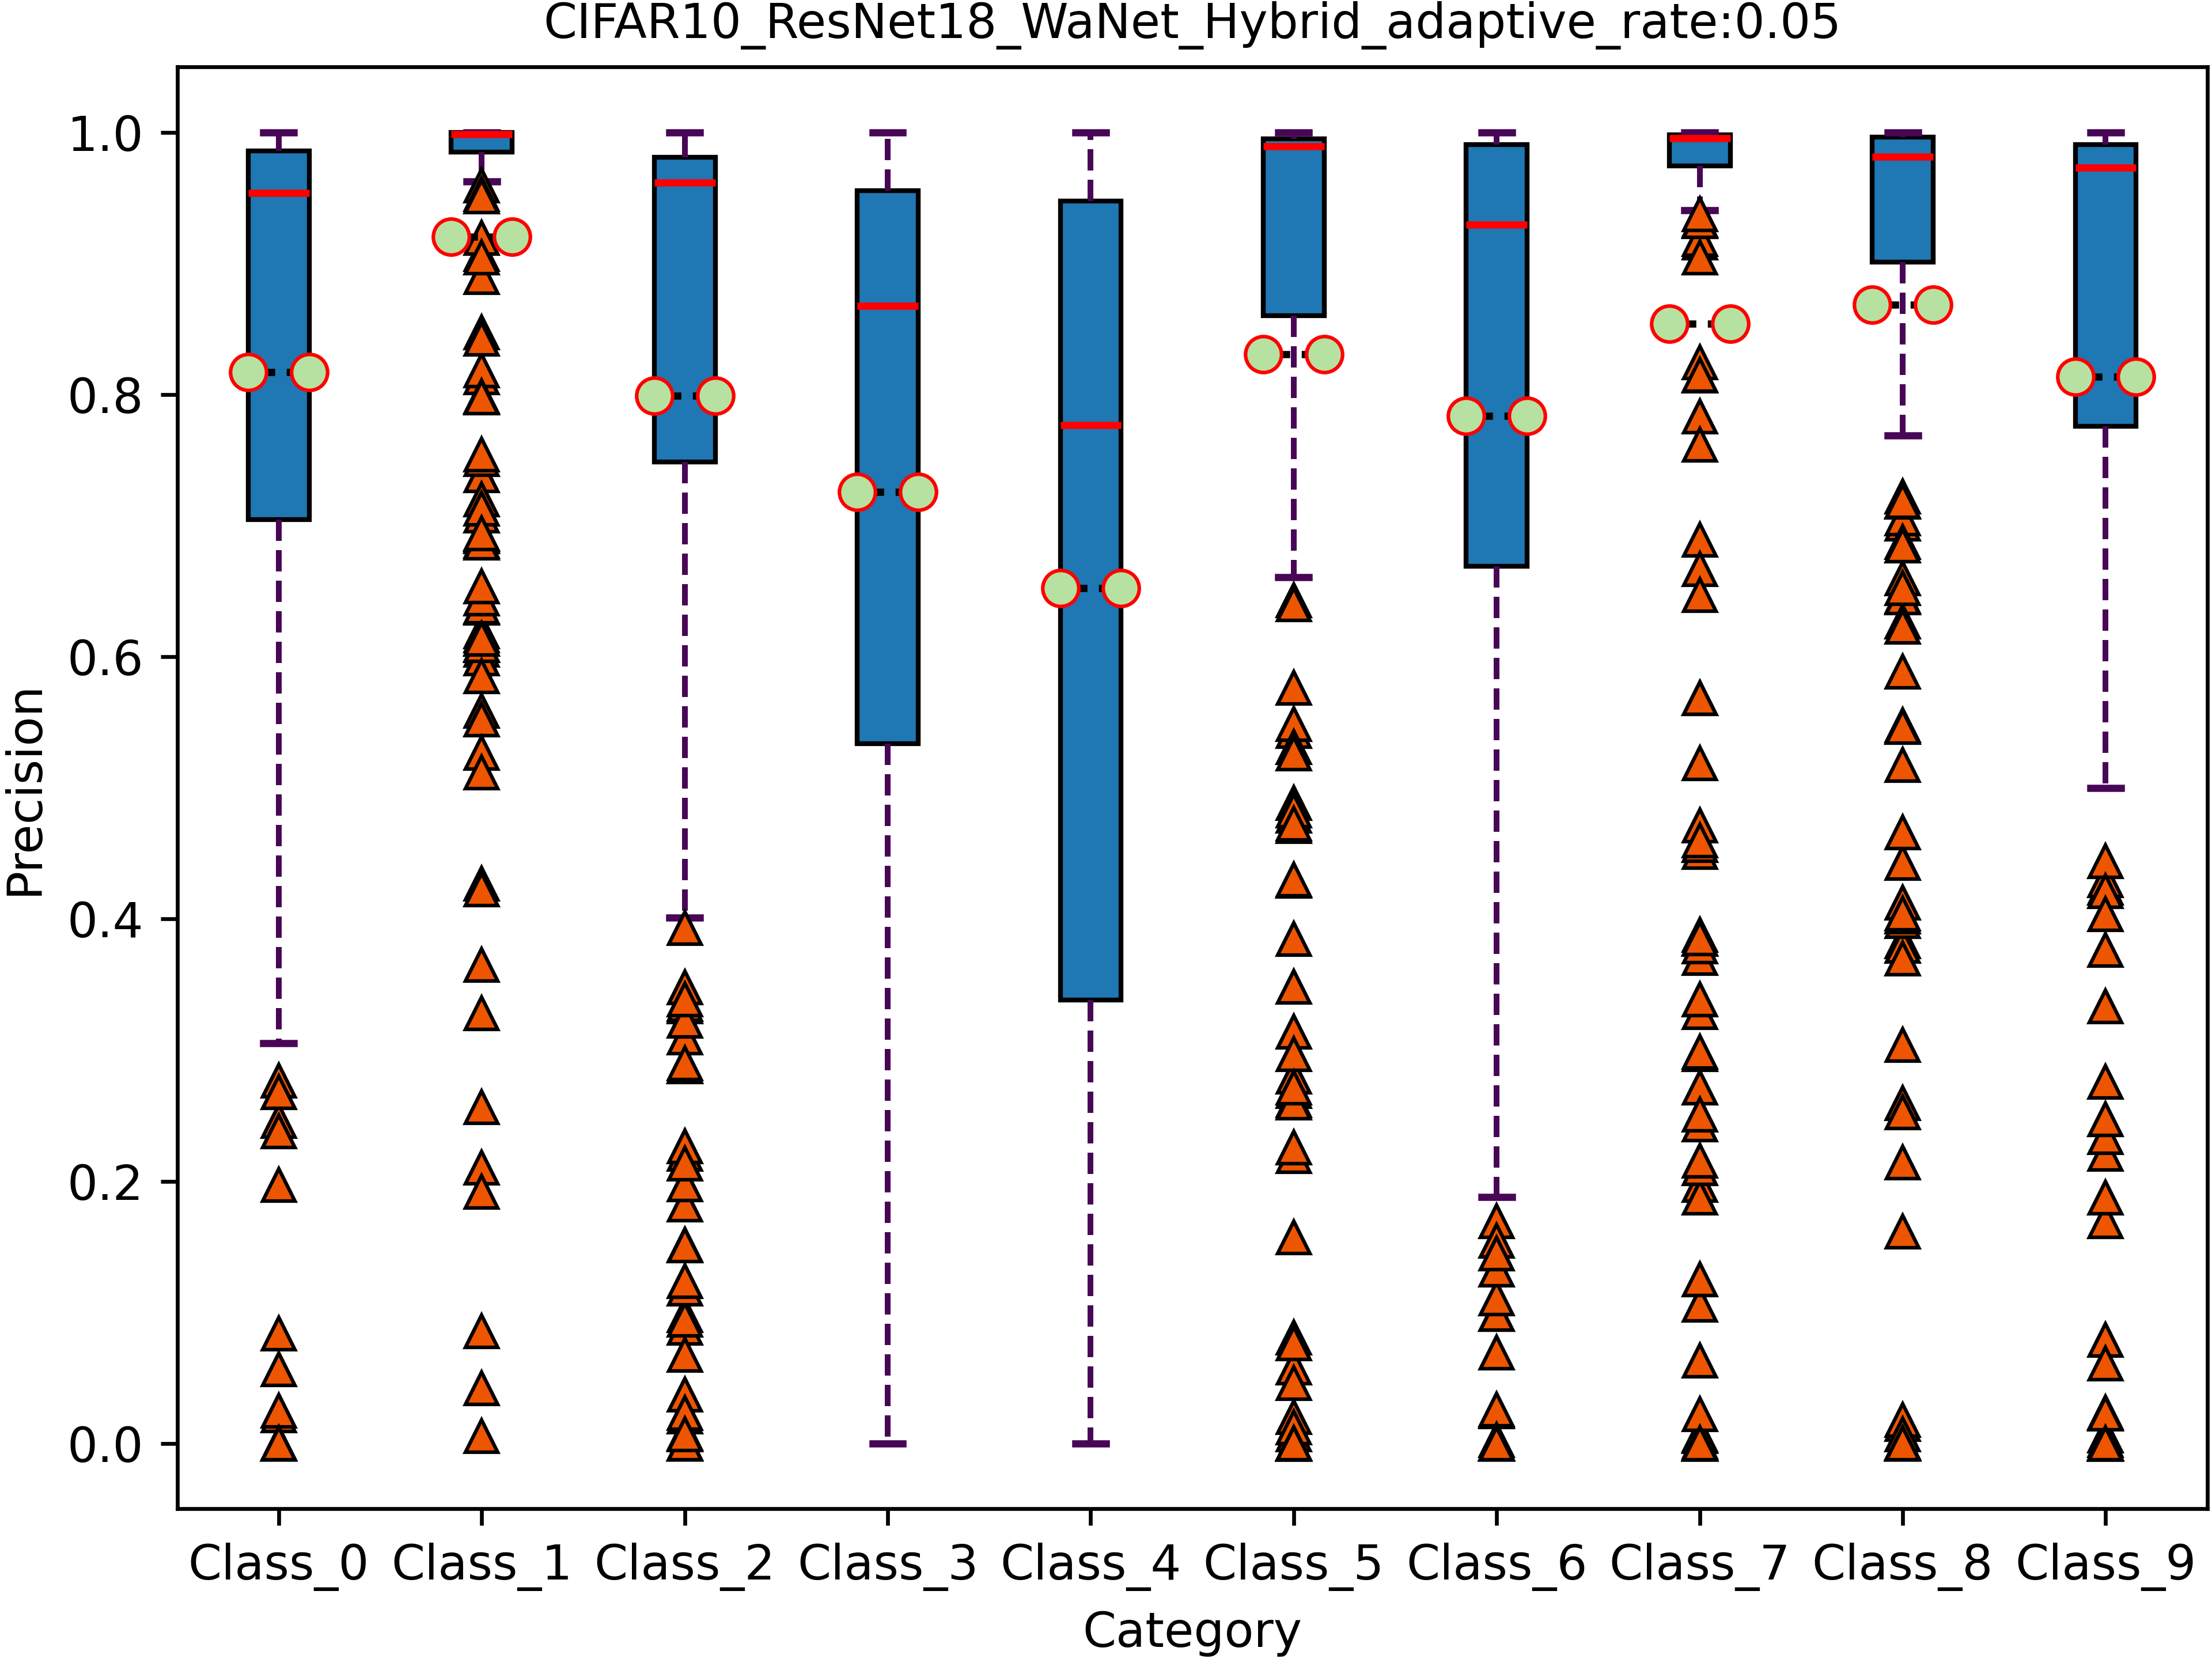
\includegraphics[scale=0.3]{./Backdoor_detect_result/target_class/WaNet.png}
		\end{minipage}
	}
	\caption{确定攻击目标类}
	\label{target_class}
\end{figure}

\begin{figure}[t]
	\subfigure[BadNets]{
		\begin{minipage}[b]{.5\linewidth}
			\centering
			\includegraphics[scale=0.1]{./Backdoor_detect_result/detect/BadNets.png}
		\end{minipage}
	}
	\subfigure[Blended]{
		\begin{minipage}[b]{.5\linewidth}
			\centering
			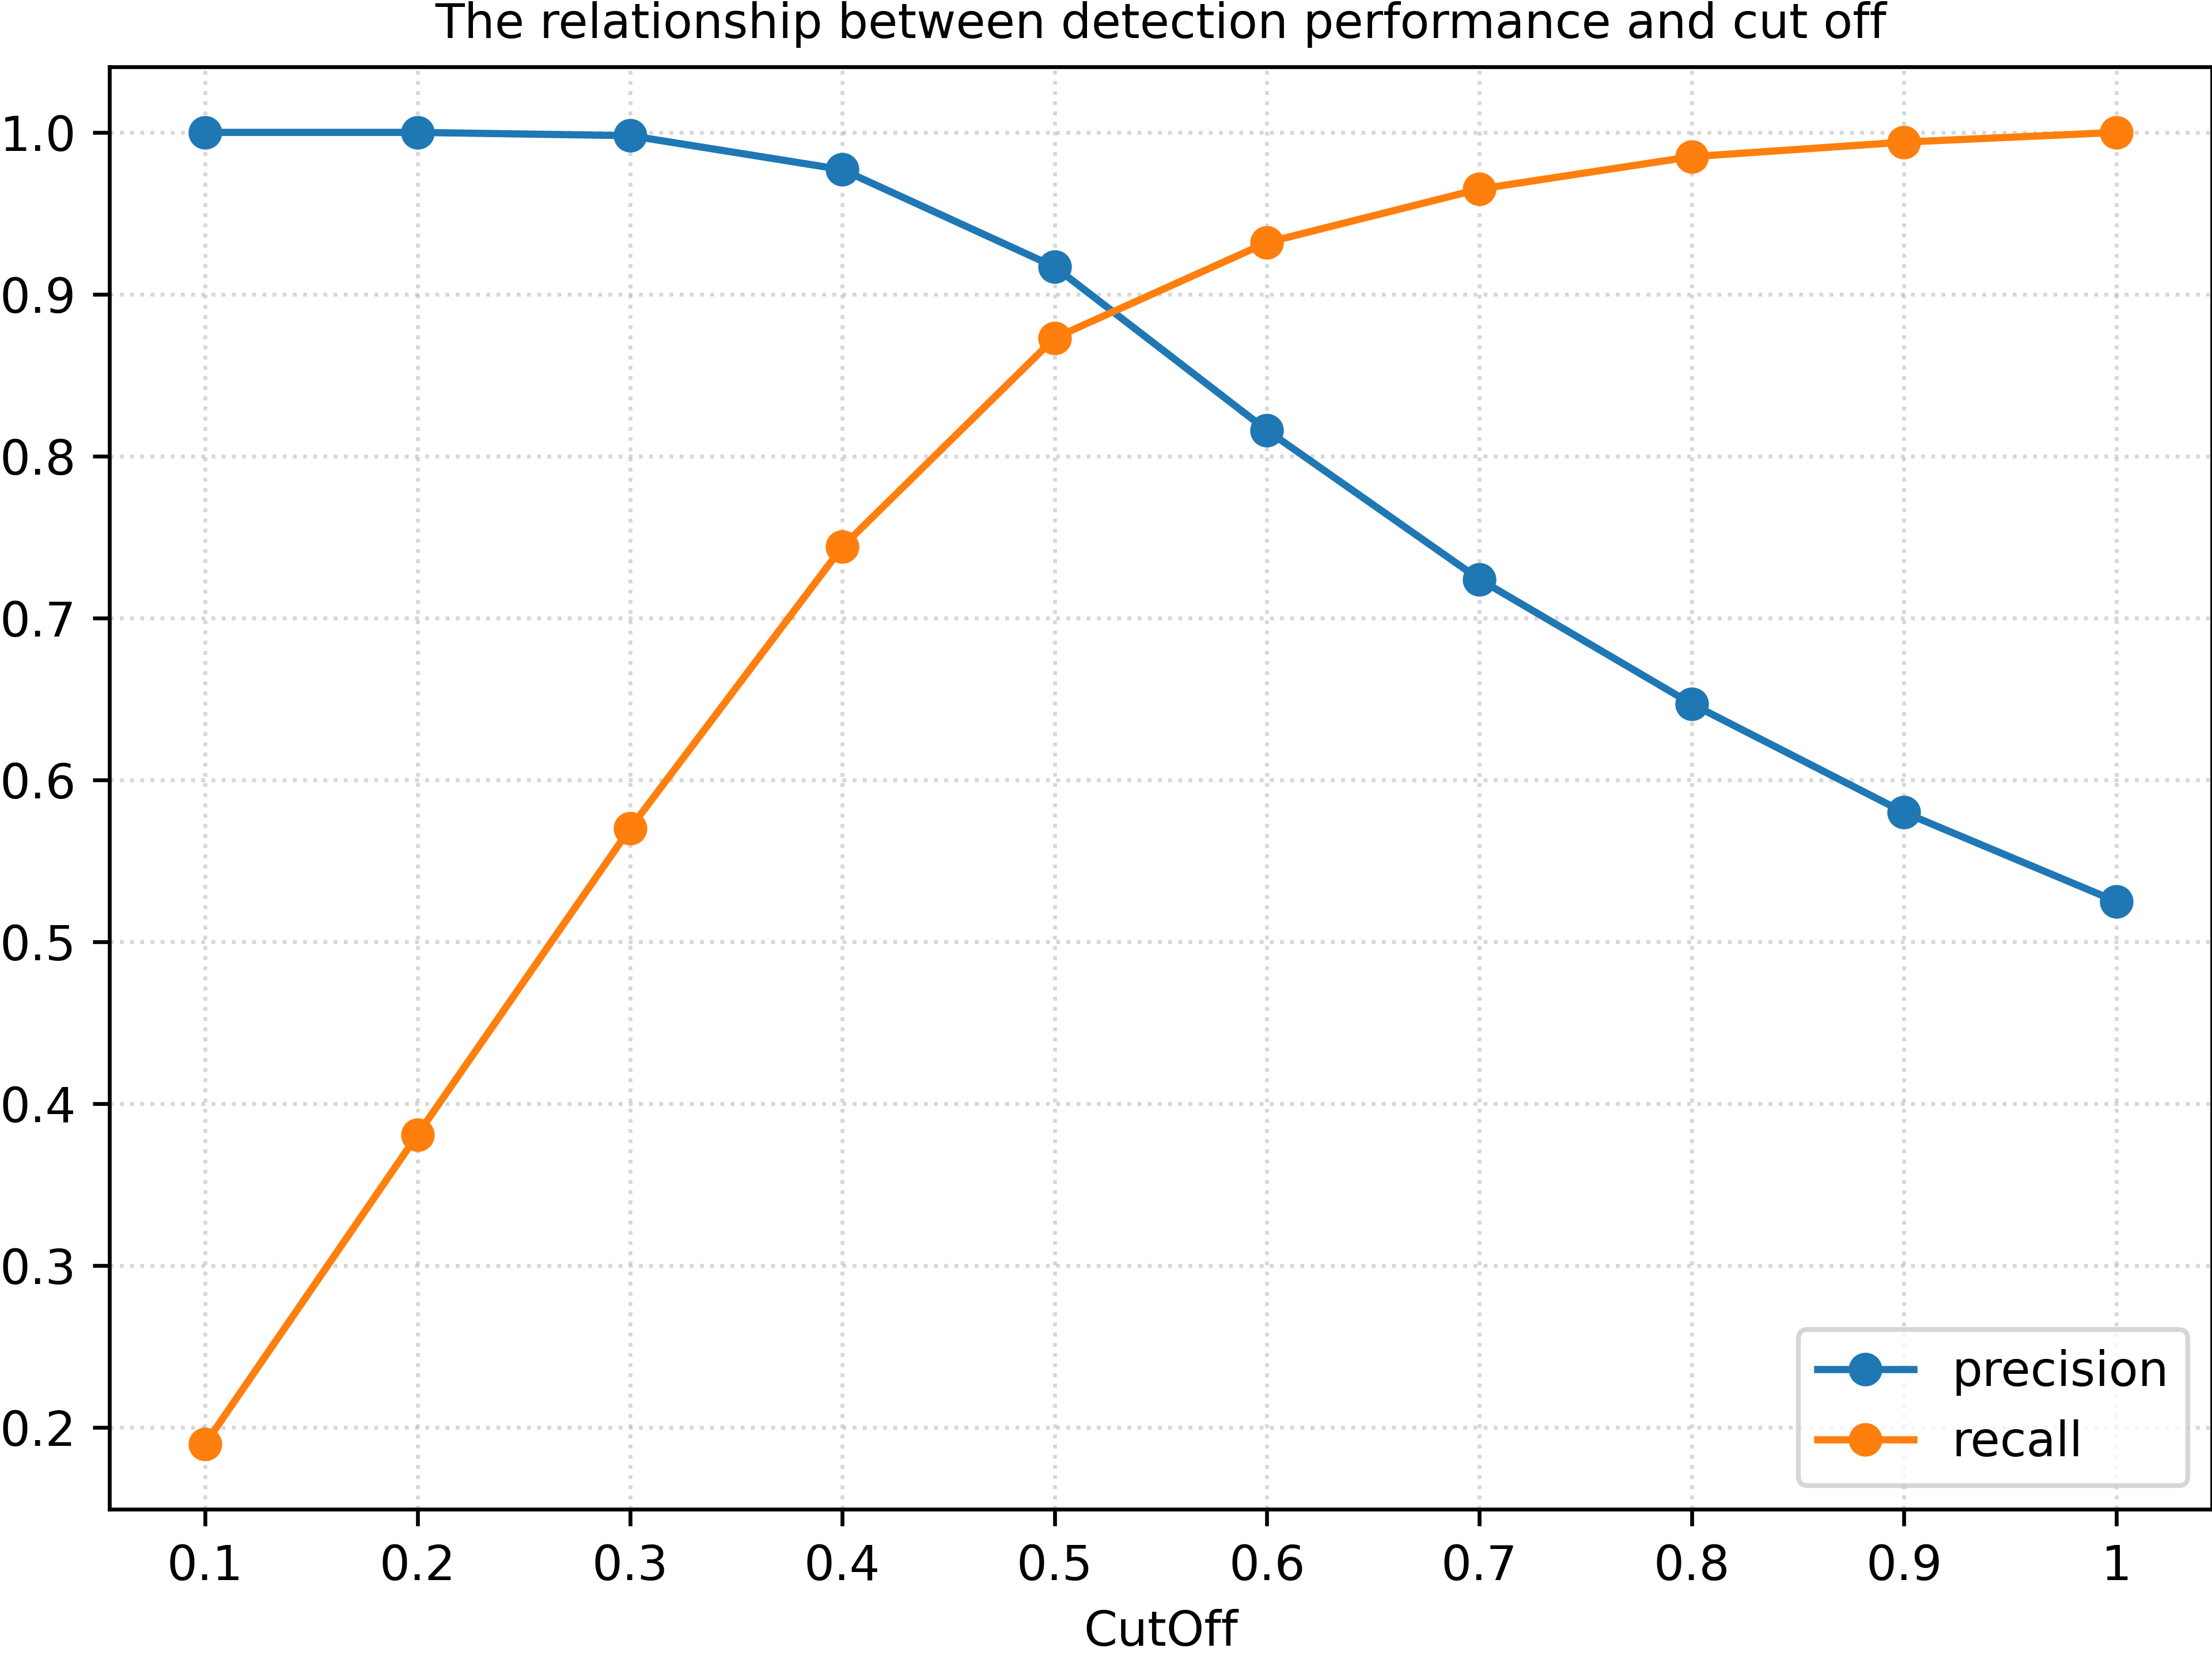
\includegraphics[scale=0.1]{./Backdoor_detect_result/detect/Blended.png}
		\end{minipage}
	}
	
	\subfigure[IAD]{
		\begin{minipage}[b]{.5\linewidth}
			\centering
			\includegraphics[scale=0.1]{./Backdoor_detect_result/detect/IAD.png}
		\end{minipage}
	}
	\subfigure[LabelConsistent]{
		\begin{minipage}[b]{.5\linewidth}
			\centering
			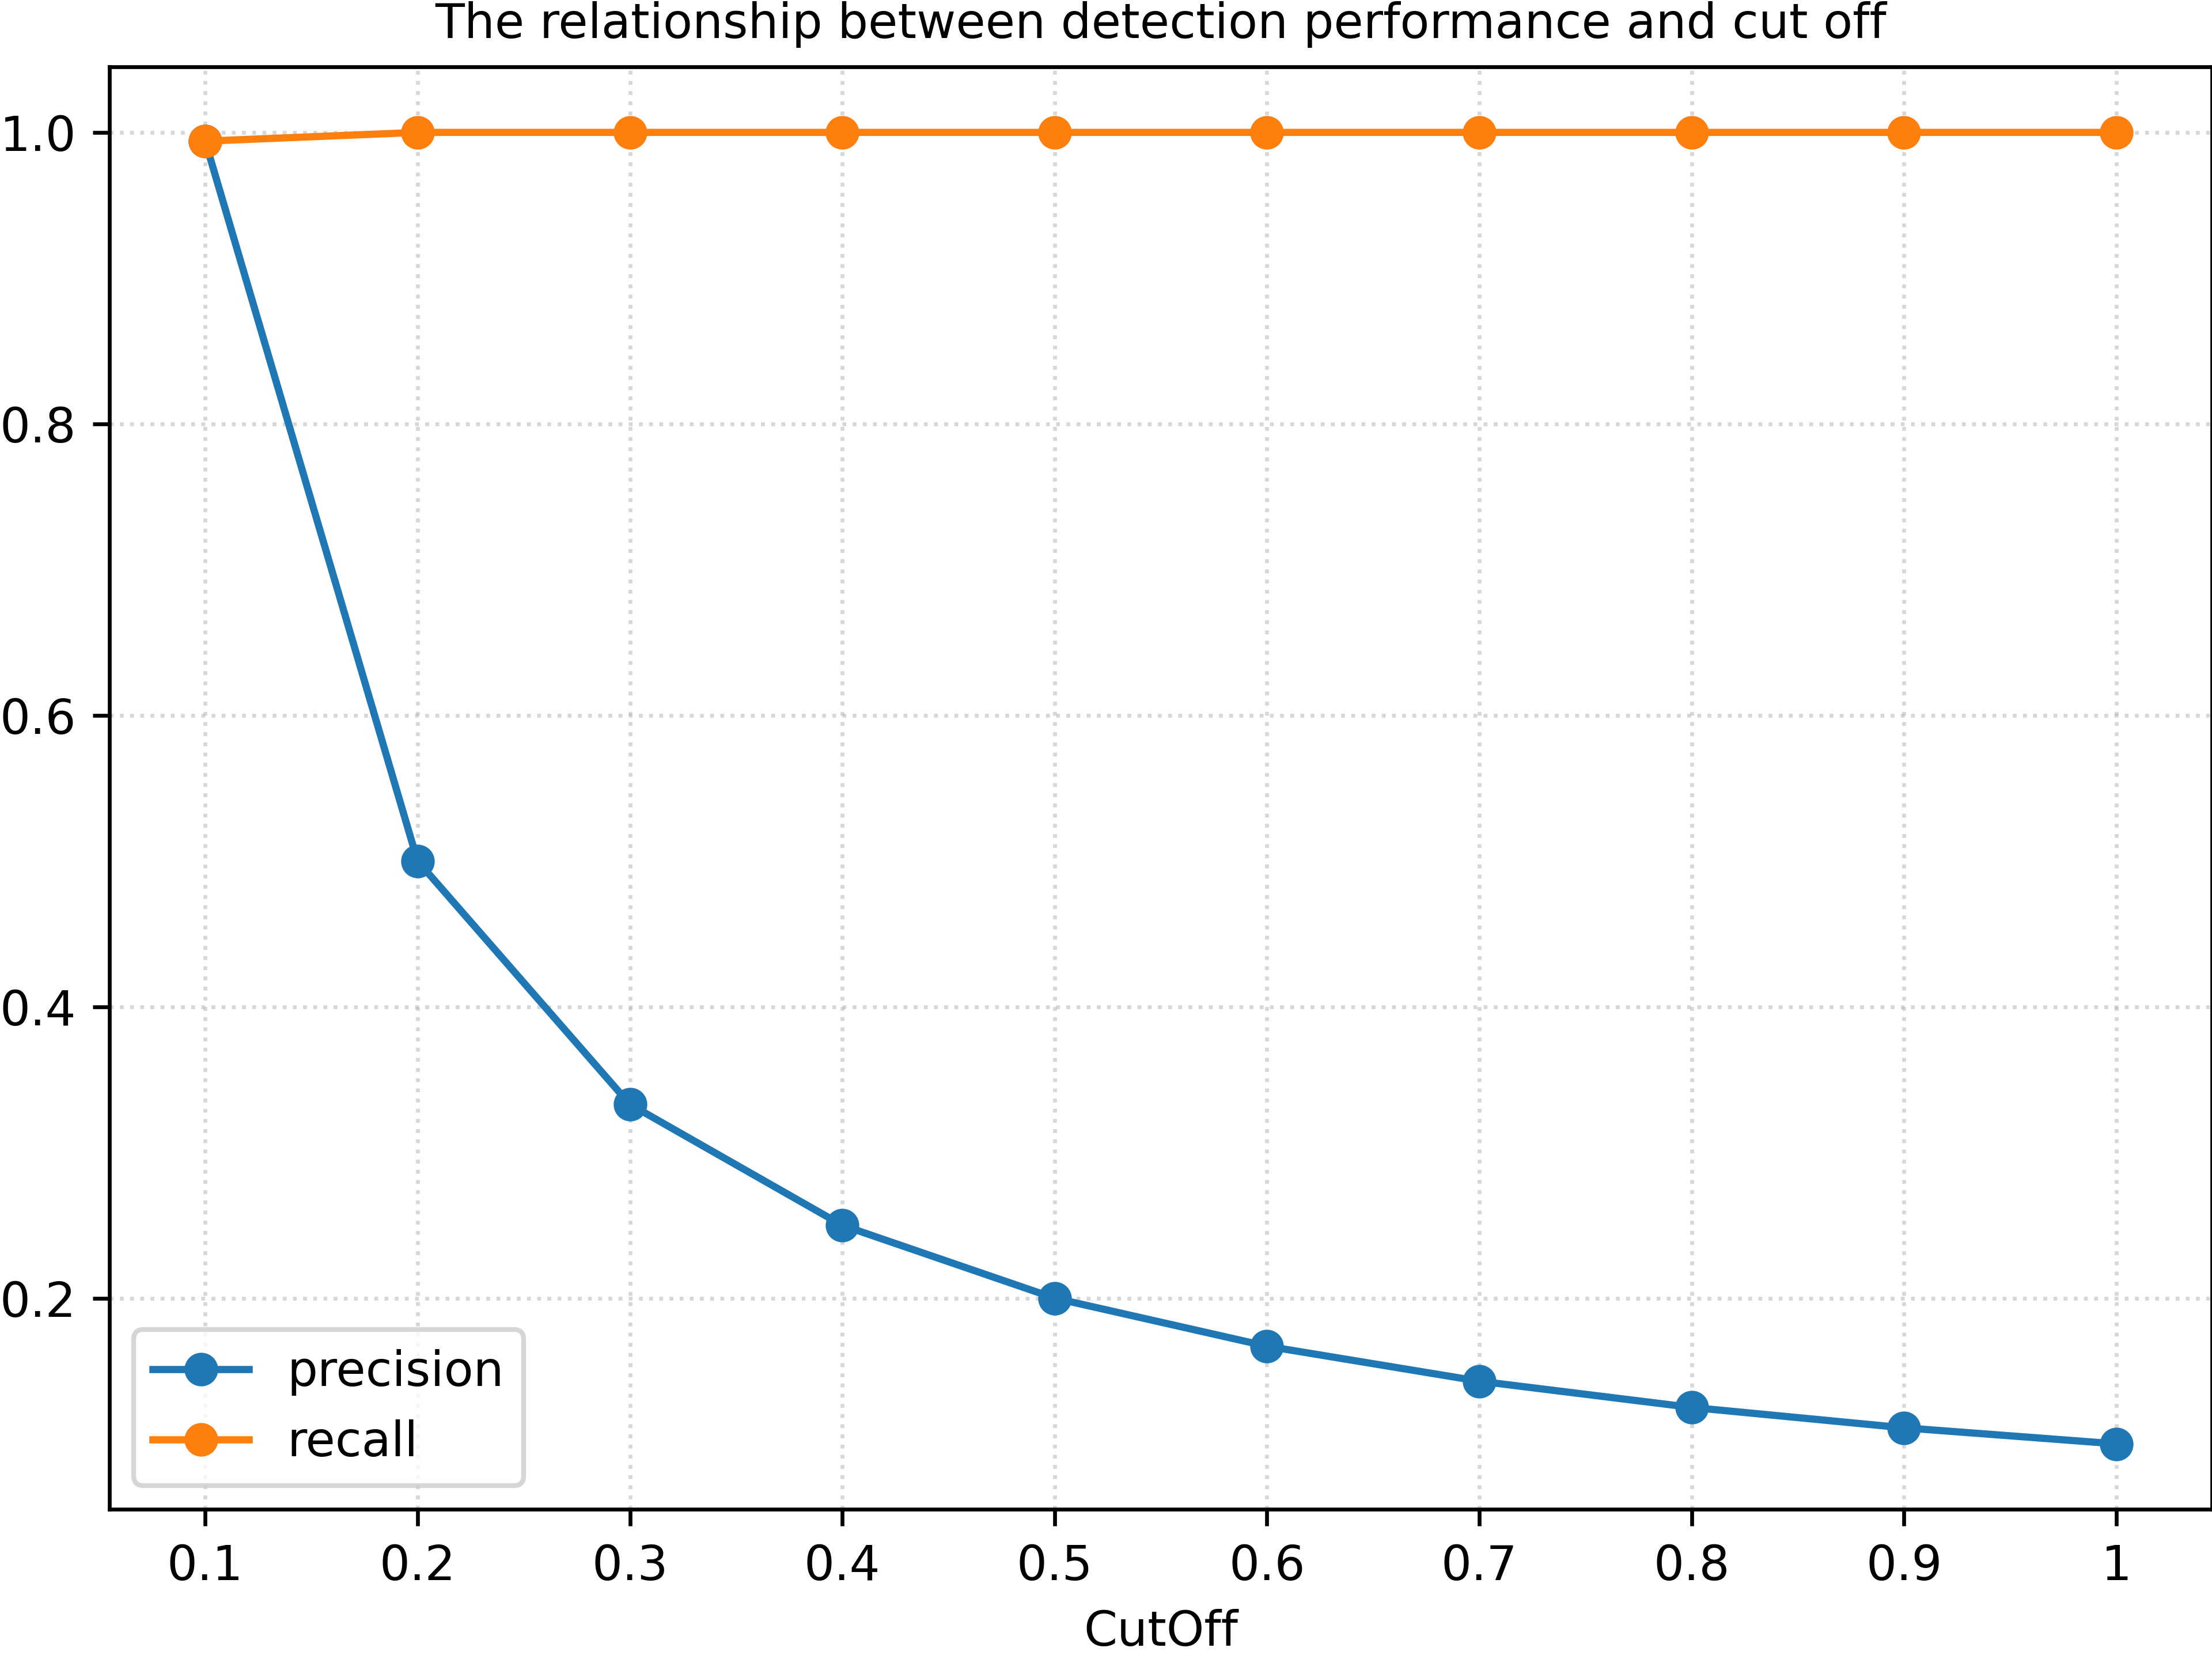
\includegraphics[scale=0.1]{./Backdoor_detect_result/detect/LabelConsistent.png}
		\end{minipage}
	}
	
	\subfigure[Refool]{
		\begin{minipage}[b]{.5\linewidth}
			\centering
			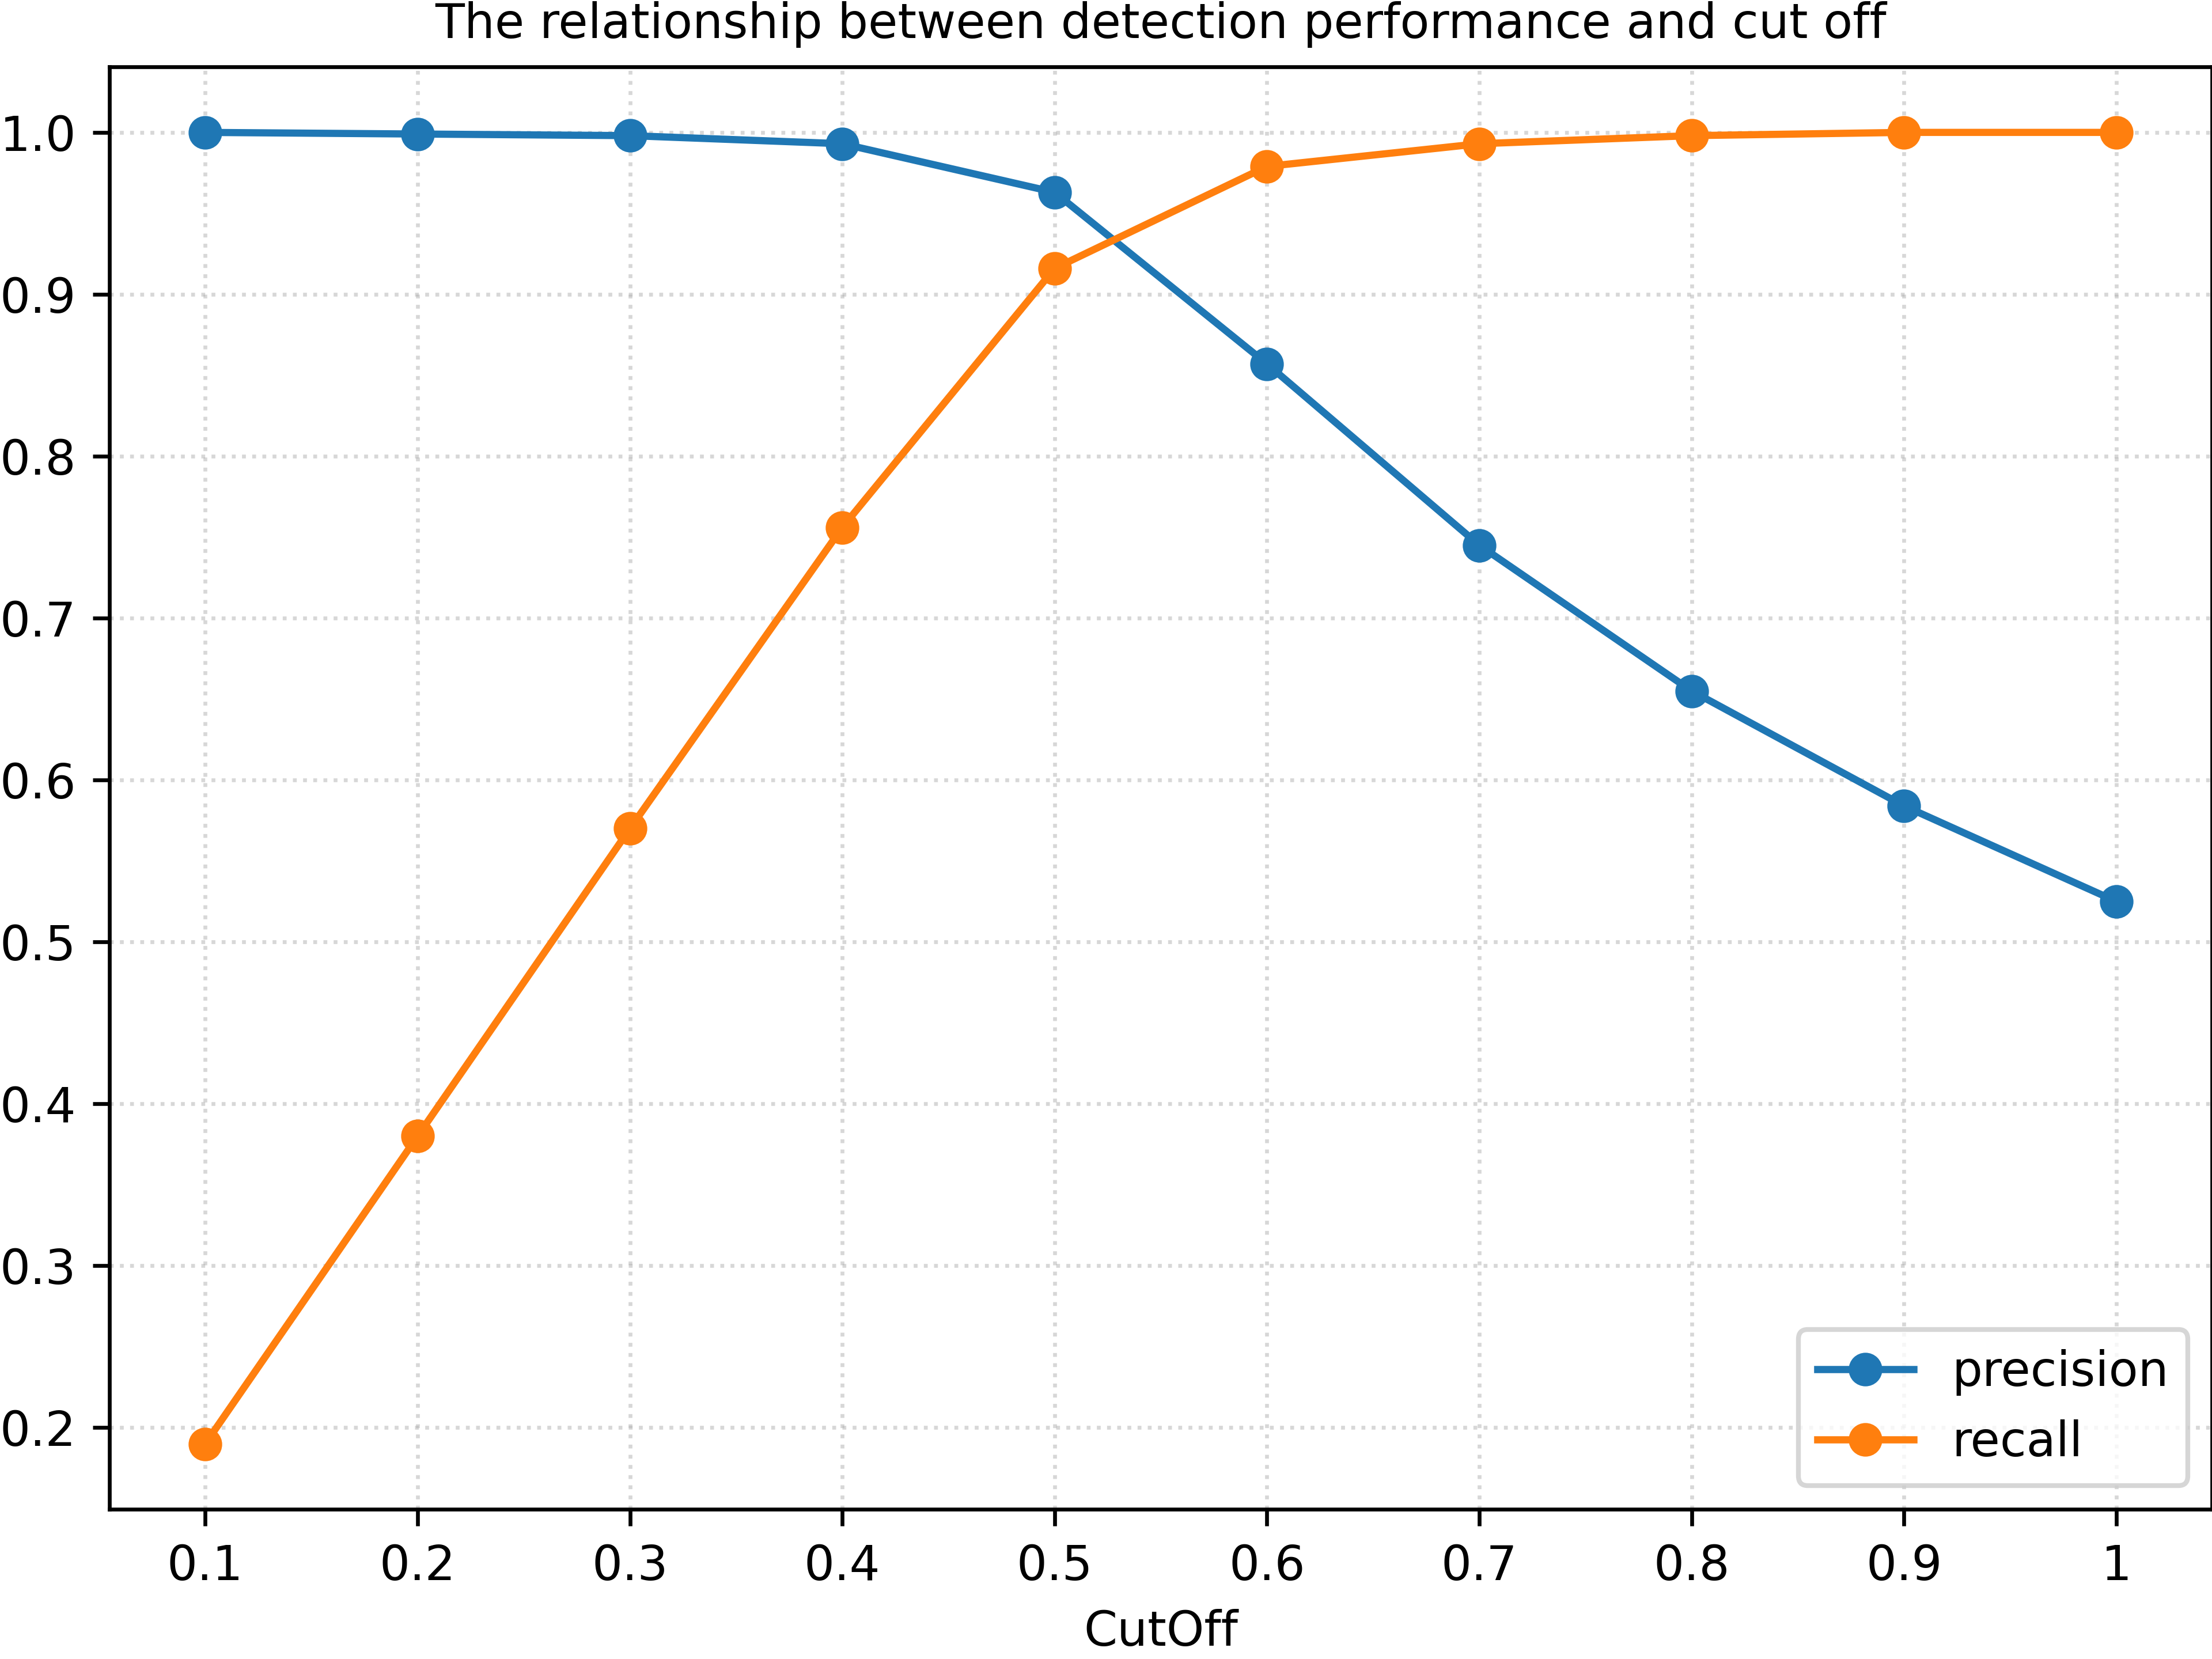
\includegraphics[scale=0.1]{./Backdoor_detect_result/detect/Refool.png}
		\end{minipage}
	}
	\subfigure[WaNet]{
		\begin{minipage}[b]{.5\linewidth}
			\centering
			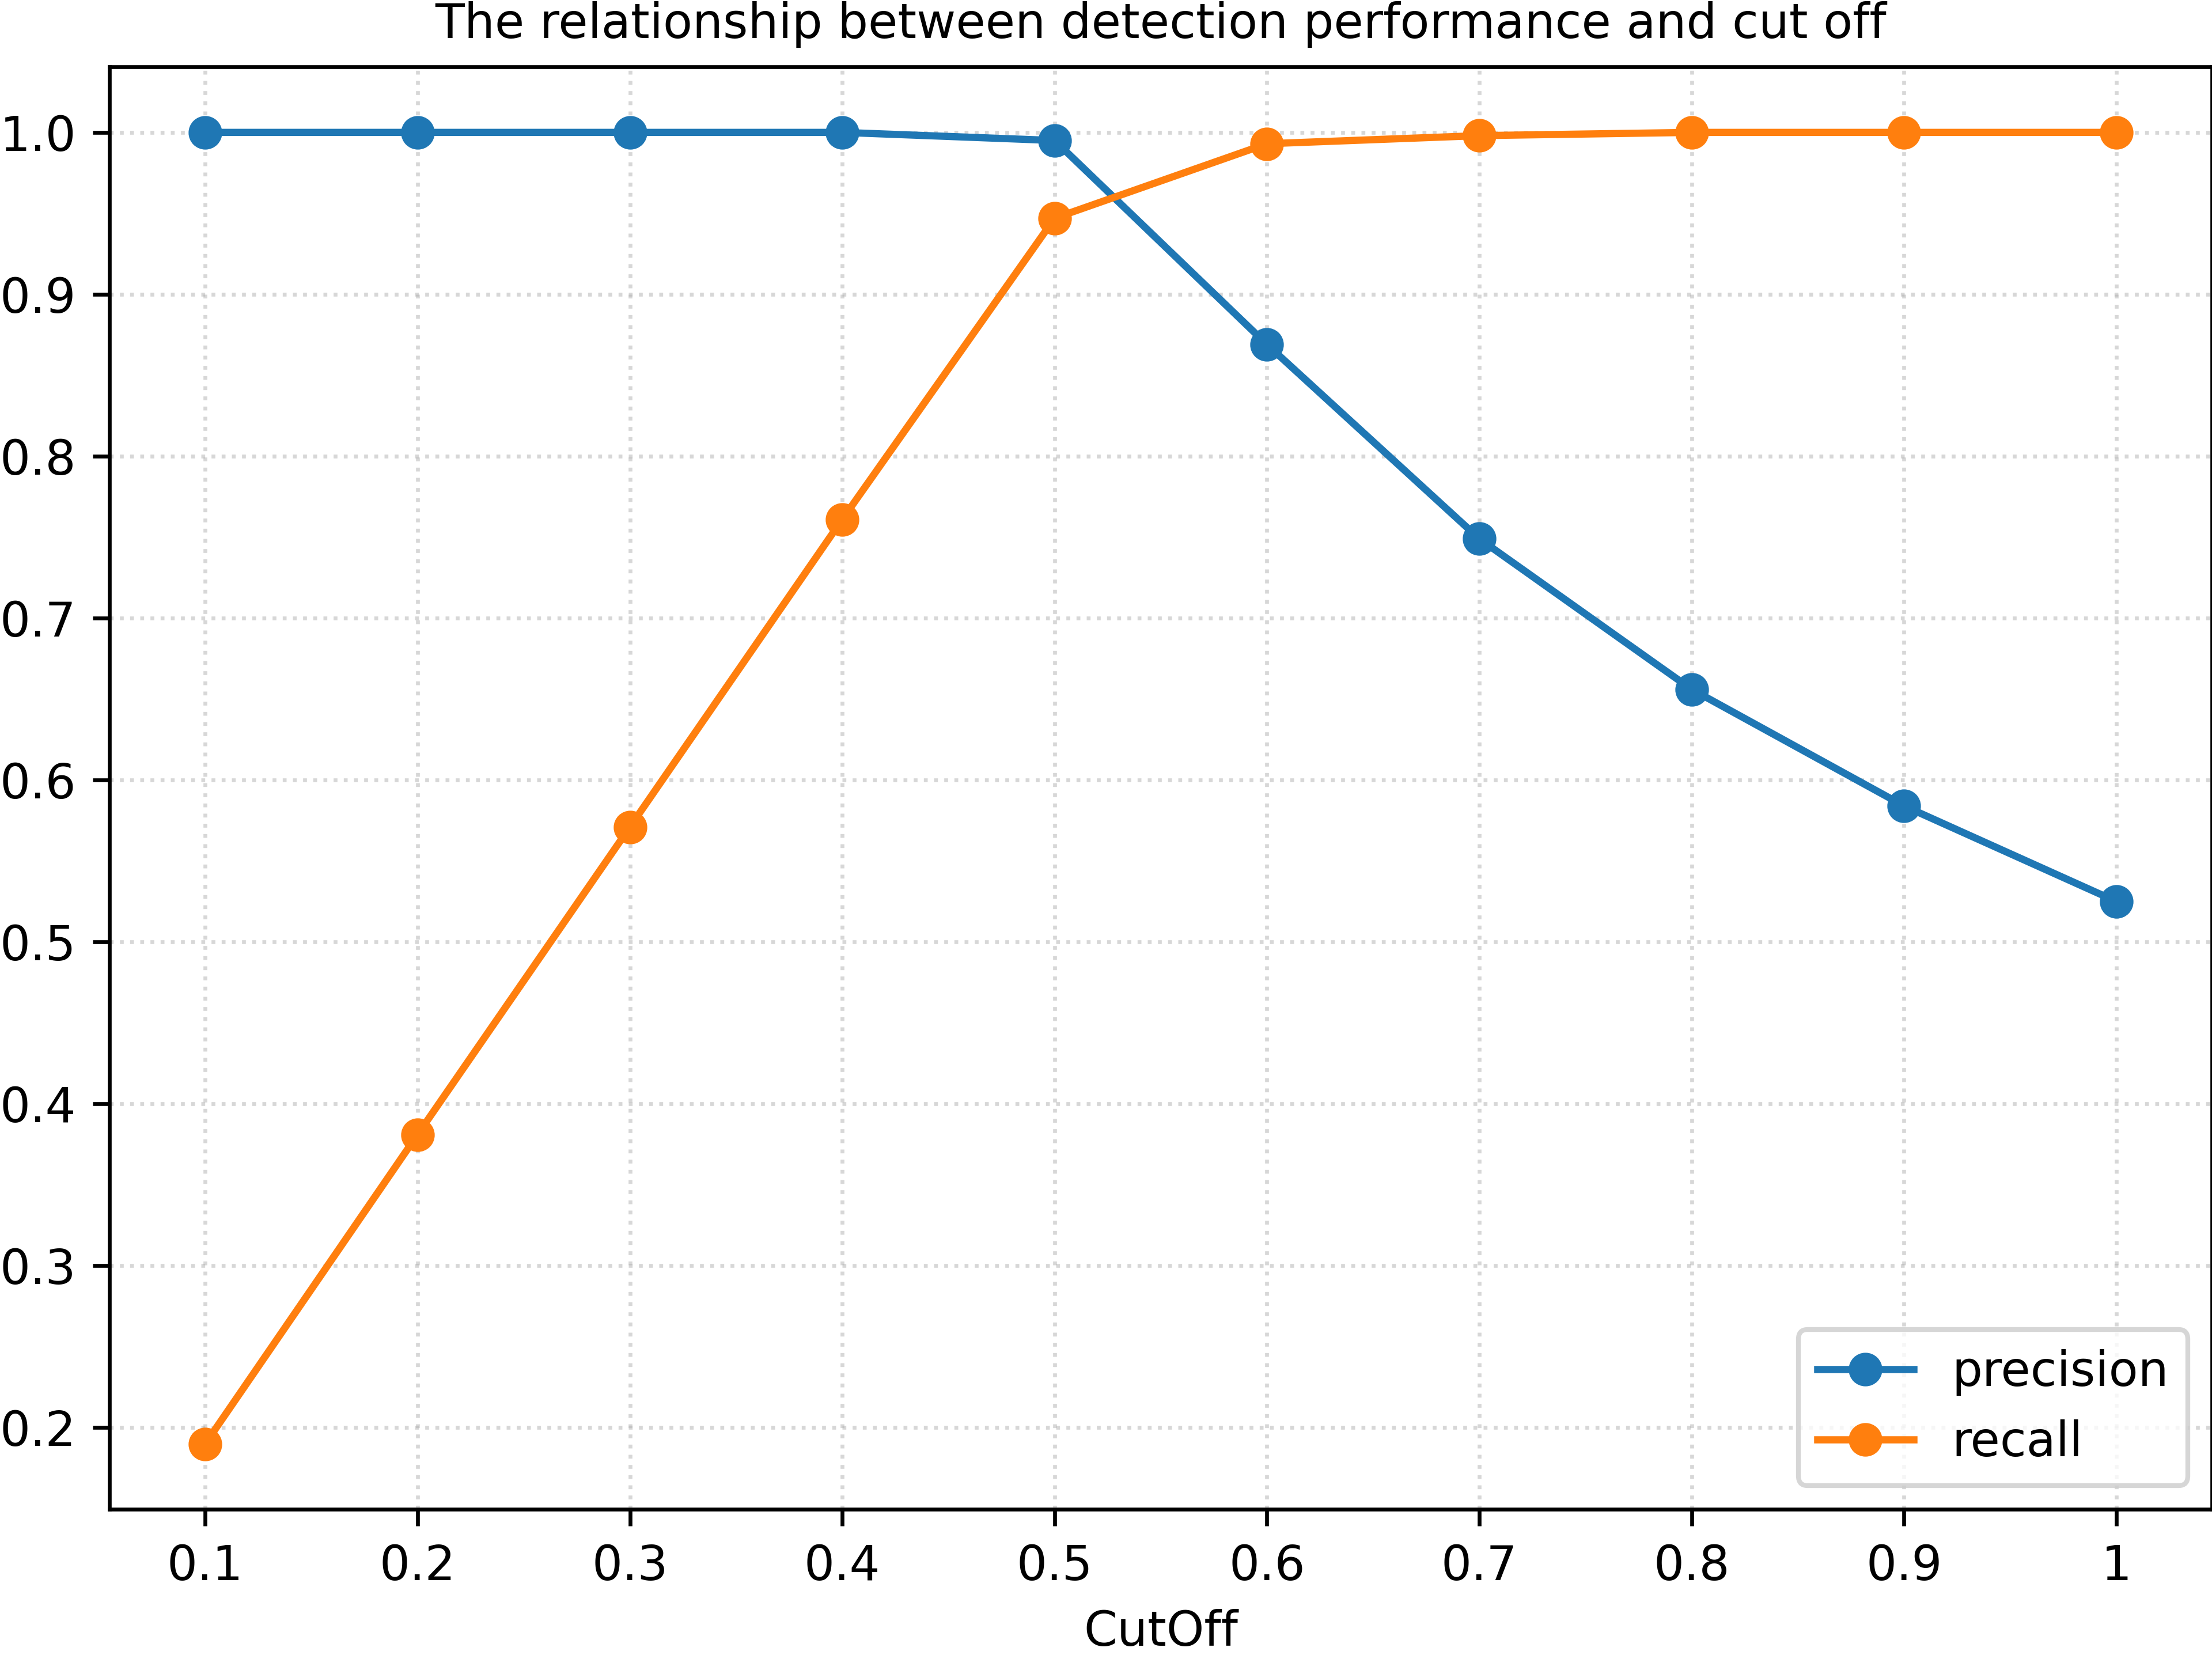
\includegraphics[scale=0.1]{./Backdoor_detect_result/detect/WaNet.png}
		\end{minipage}
	}
	
	\caption{确定攻击目标类}
	\label{detect}
\end{figure}


\section{之前工作总结和未来工作展望}

目前我们的工作专注于深度学习模型融合与测试技术研究,解决了两个相关的研究问题: 1)模型融合; 2)木马输入检测。对于模型融合研究,考虑了一种新的应用场景。如何复用功能重叠的模型,在受限的标记代价下如何能够提高模型的分类性能,提出了一种新的基于级联并行的模型合并技术,通过复用已有模型,来提高开发效率。对于深度学习模型的测试技术研究,我们利用变异测试技术,提出一种新的测试方法用于检测木马输入。

未来的工作会继续关注深度学习模型融合和测试技术研究。在模型融合技术研究方面,如软件分类需求变更过程中,需要对某个分类做出更细的分类,“如何对现有模型进行融合并在有限标记代价下满足新的需求”将是我们研究的重点。对于模型测试技术继续探索如何使用变异测试修复和移除隐藏在模型的后门。由于目前的研究主要聚焦在图片分类数据集上,未来会评估我们的方法在不同的数据集上,如自然语言处理数据集,这将使我们的研究可以覆盖到更多的应用领域。
\begin{comment}
	\begin{tabular}{|c|c|c|c|c|} \hline % 其中,|c|表示文本居中,文本两边有竖直表线。
		$\mathcal{M}_a$ & $\mathcal{M}_b$ & $\mathcal{M}_c$ & score \\ \hline
		\checkmark & \checkmark & \checkmark & 4 \\ \hline
		\checkmark & \checkmark &$ \times $ & 3  \\ \hline
		\checkmark & $\times$ & \checkmark  & 3  \\ \hline
		$\times$ & \checkmark & \checkmark  & 2  \\ \hline
		$\times$ & $\times$ & $\times$  & 0  \\ \hline
	\end{tabular}
	
	\begin{tabular}{|c|c|c|} \hline % 其中,|c|表示文本居中,文本两边有竖直表线。
		场景 & 4分精度 & 3分精度  \\ \hline
		Food & 97.7\% & 74.3\%  \\ \hline
		Sport & 98.36\% &69.82\%   \\ \hline
		Animal & 92.98\% & 79.48\%  \\ \hline
		Weather & 91.48\% & 70.48\%   \\ \hline
	\end{tabular}
\end{comment}

\bibliographystyle{plain}
\bibliography{ref}

\end{document}
